\section{Calibration}
This section focuses on the calibration of the Rasperry Pi Camera Module V2 (resolution set to $3280\times 2464$\,pixels),
but all insights learned from these first attempts are applicable to the similar (but higher quality) cameras, which where later also used.

To capture the whole steel-spring, the camera has to be mounted approximately 250\,mm away from it.
From this distance, one pixel-width corresponds to a length within the tenths of a millimeter range.
It is therefore absolutely necessary to calibrate the camera as described in section \ref{theory:calibration}, since non-linear distortions can distort the image by 10-20\, pixels or even more.
Lens imperfections can therefore cause deviations in the measurement of several millimeters, which is not acceptable.

To calibrate a camera in OpenCV, one has to take images of a known 2D-pattern.
It is reasonable to use a checkerboard, since OpenCV provides functions to detect checkerboard-corners reliably with subpixel precision.

\subsection{Calibration statistics\label{development:statistics}}
First attempts to calibrate the camera failed.
Despite reprojection errors of $<0.3$ pixels, the obtained distortion coefficients did not seem to deliver a good undistortion of the image.
Furthermore, new attempts with slightly different images of the checkerboard resulted in totally different coefficients. 
It is therefore important to take a closer look at the technical aspects of the calibration process.

To get more insight what went wrong, some sort of statistics is needed.
200 images of the checkerboard from different view-points and angles have been taken.
A couple of these images are shown in Figure  \ref{development:im}

\begin{figure}[ht]
	\centering
	\subfigure[\label{development:im0}]{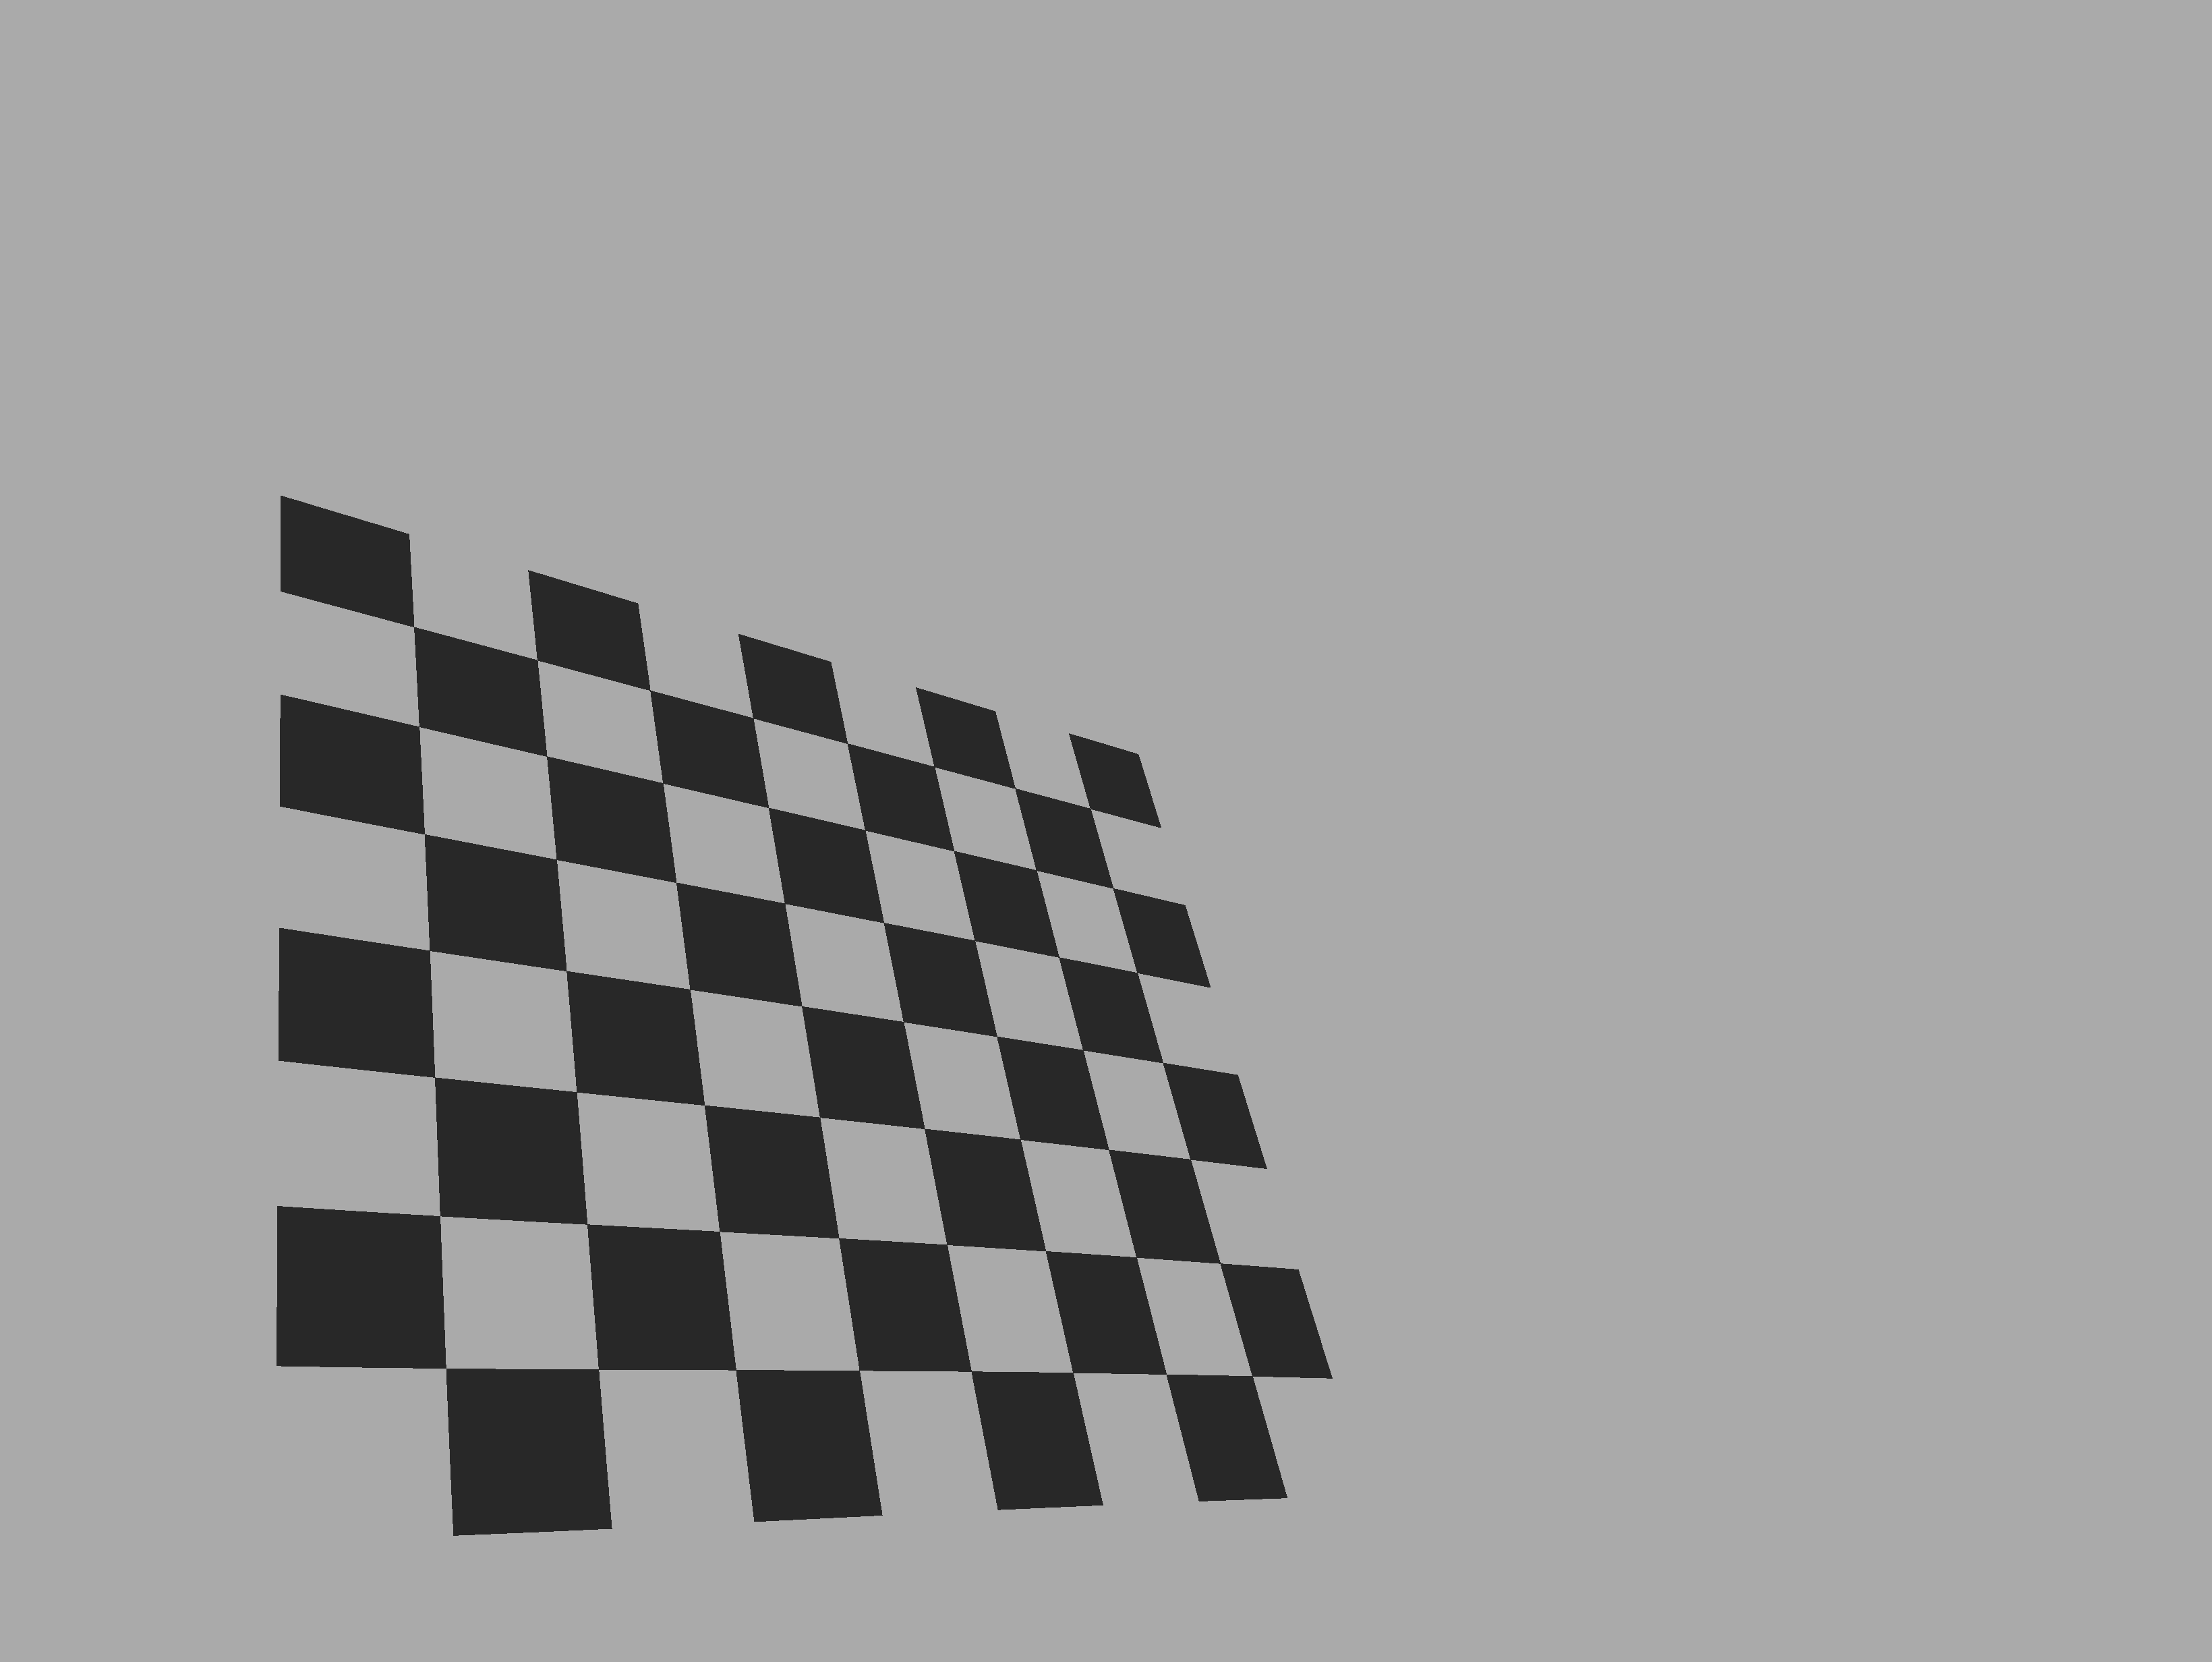
\includegraphics[width=0.3\linewidth]{3-development/calibration/images/im0.png}}
	\subfigure[\label{development:im1}]{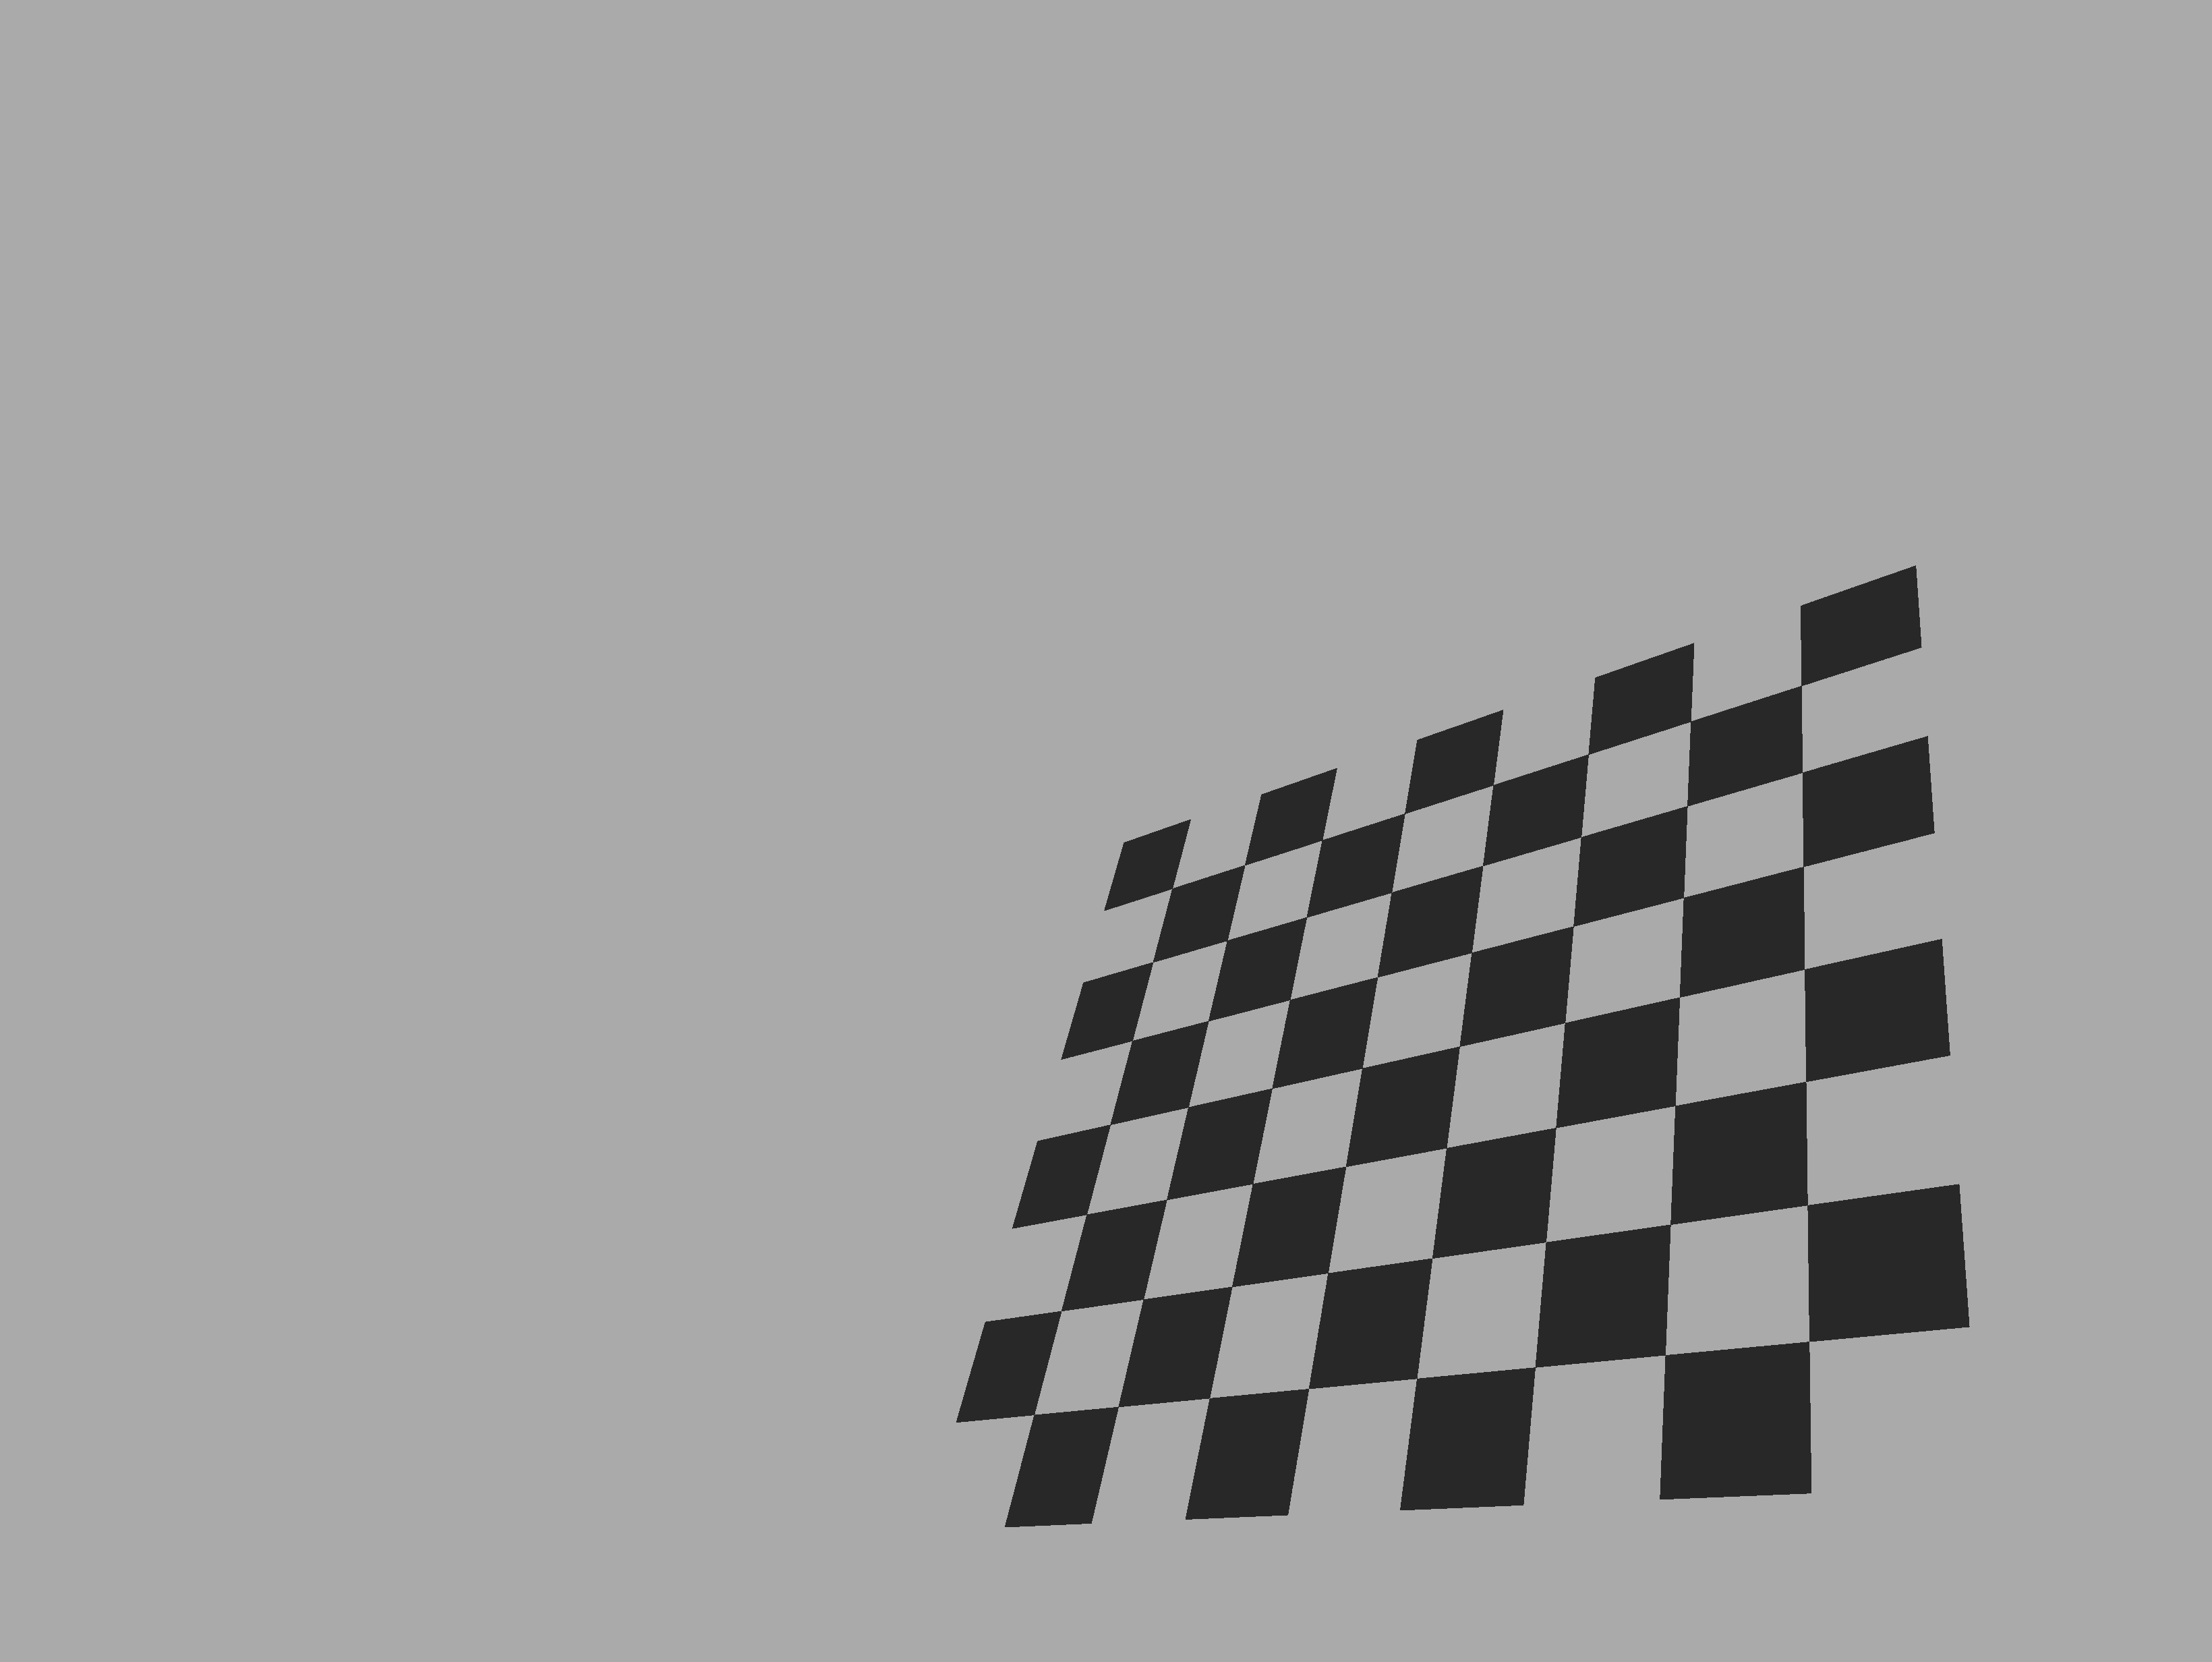
\includegraphics[width=0.3\linewidth]{3-development/calibration/images/im1.png}}
	\subfigure[\label{development:im2}]{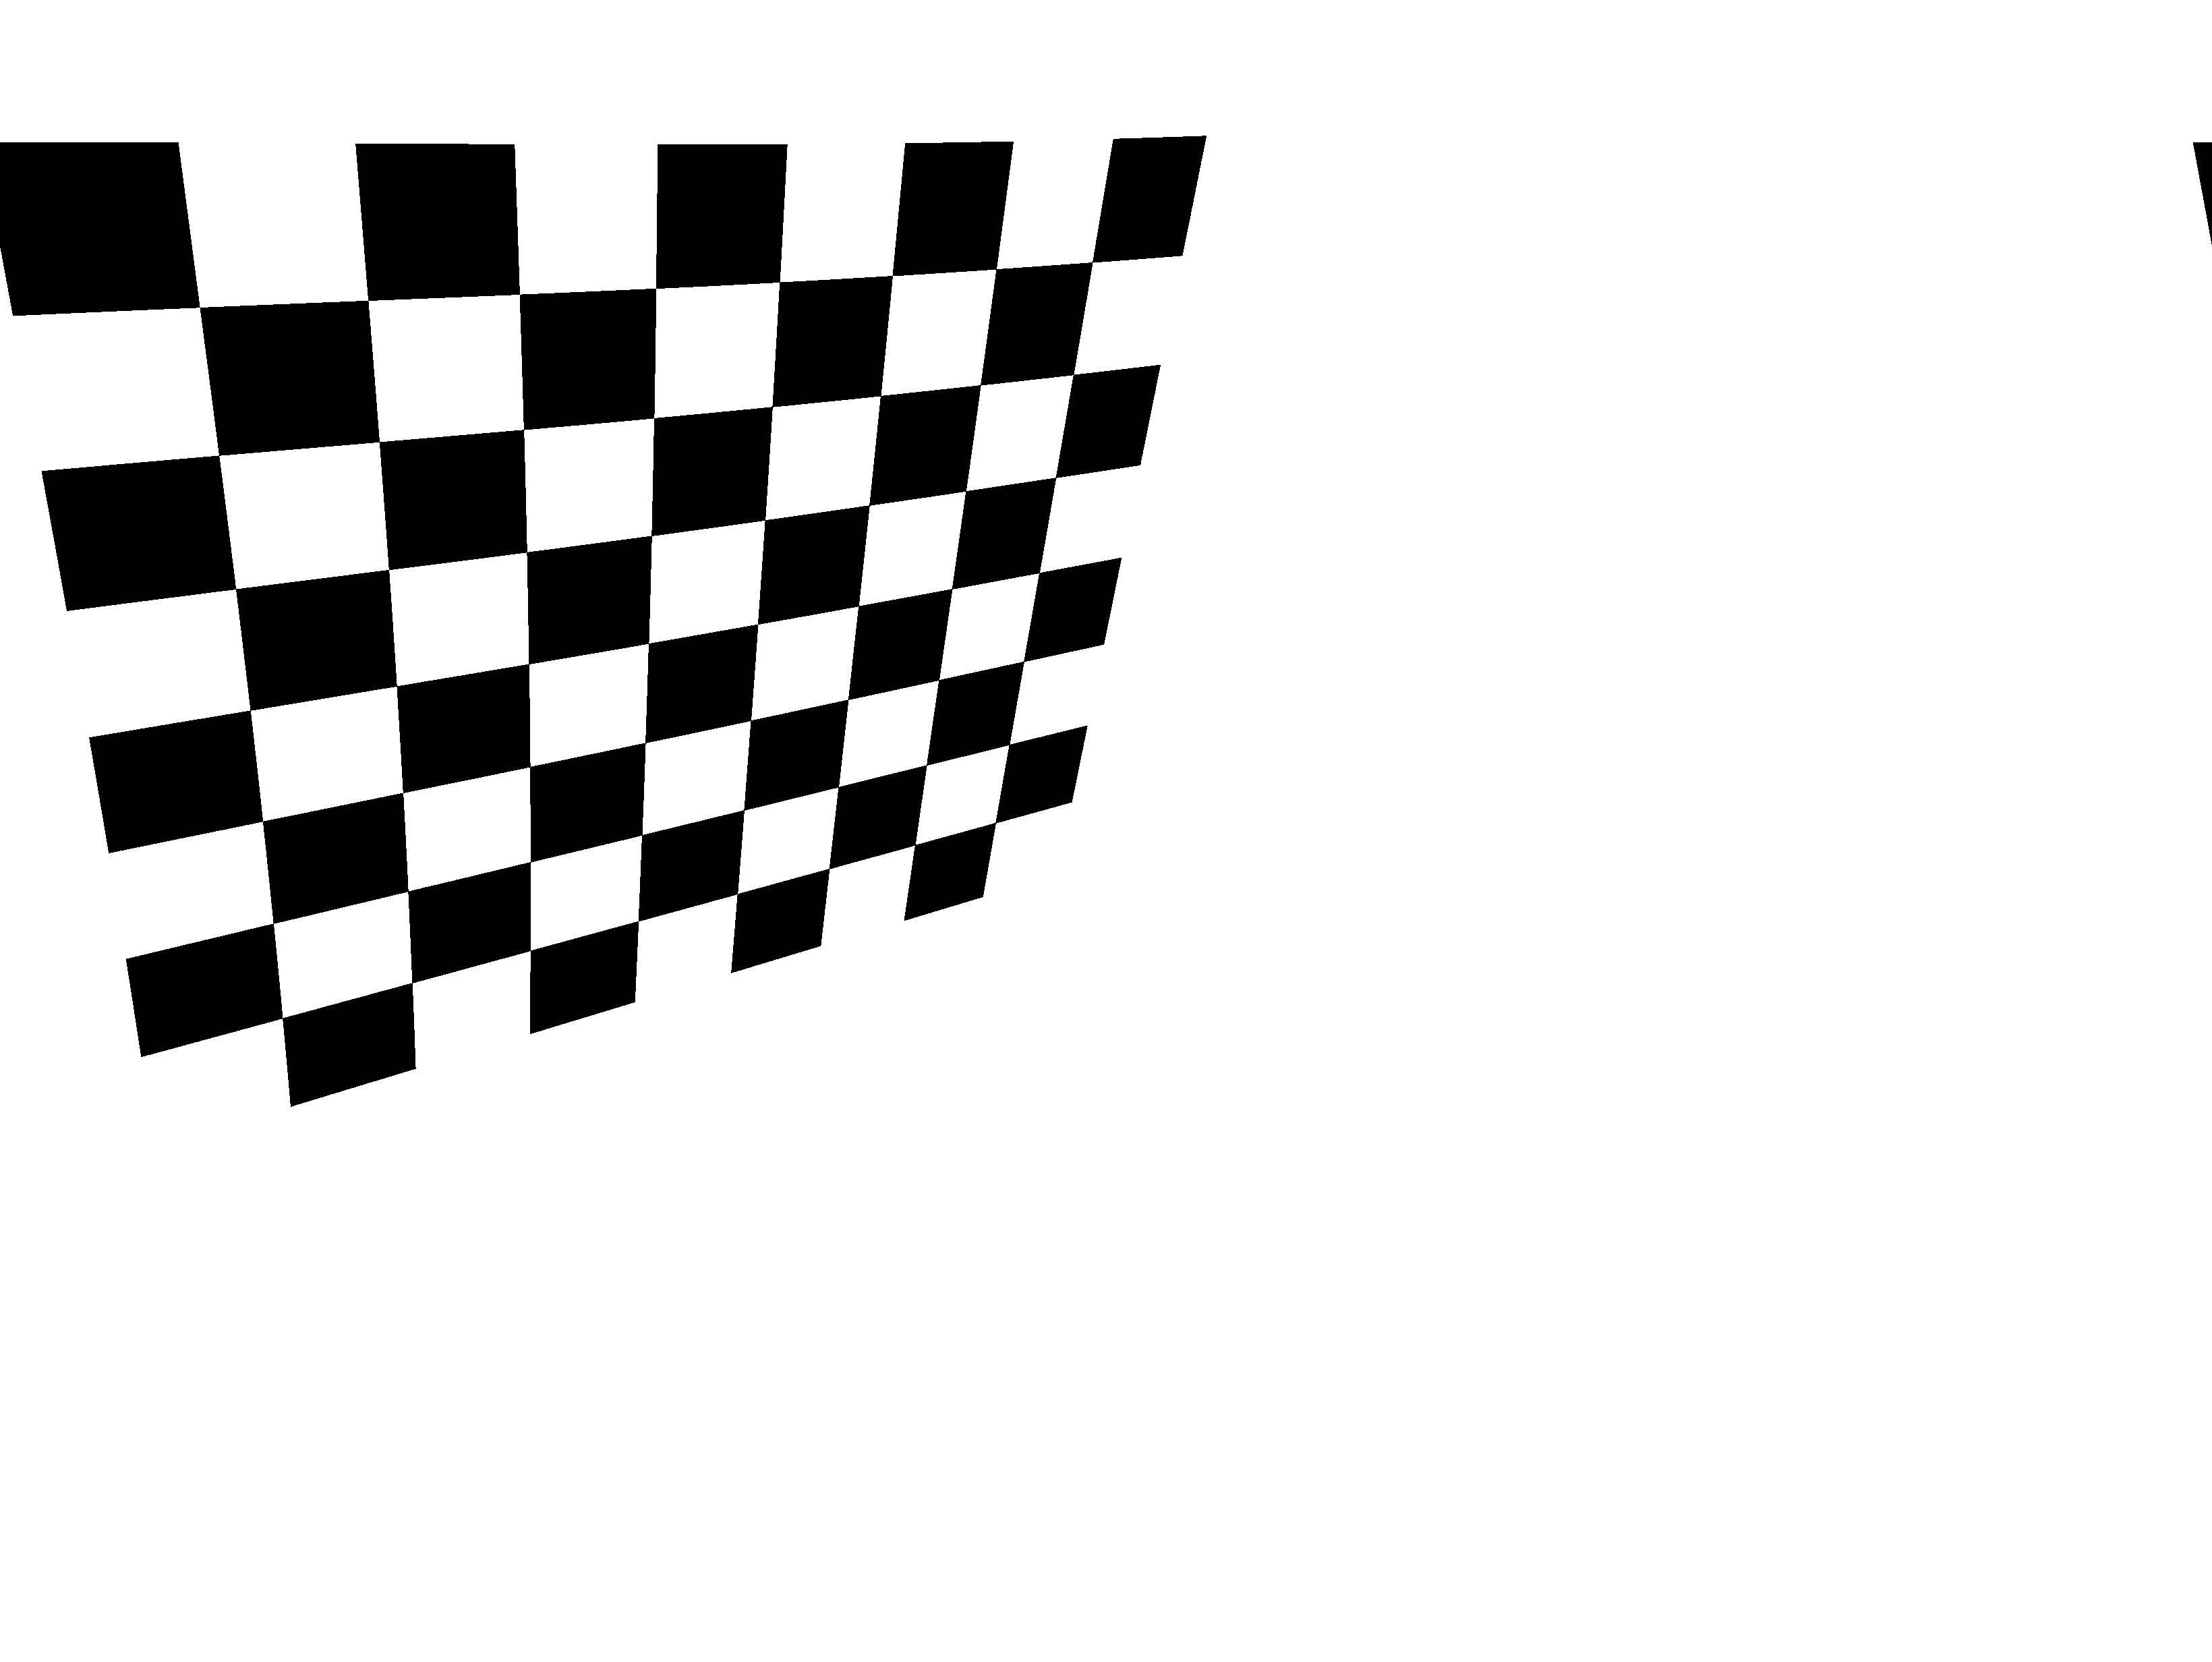
\includegraphics[width=0.3\linewidth]{3-development/calibration/images/im2.png}}
	
	\subfigure[\label{development:im3}]{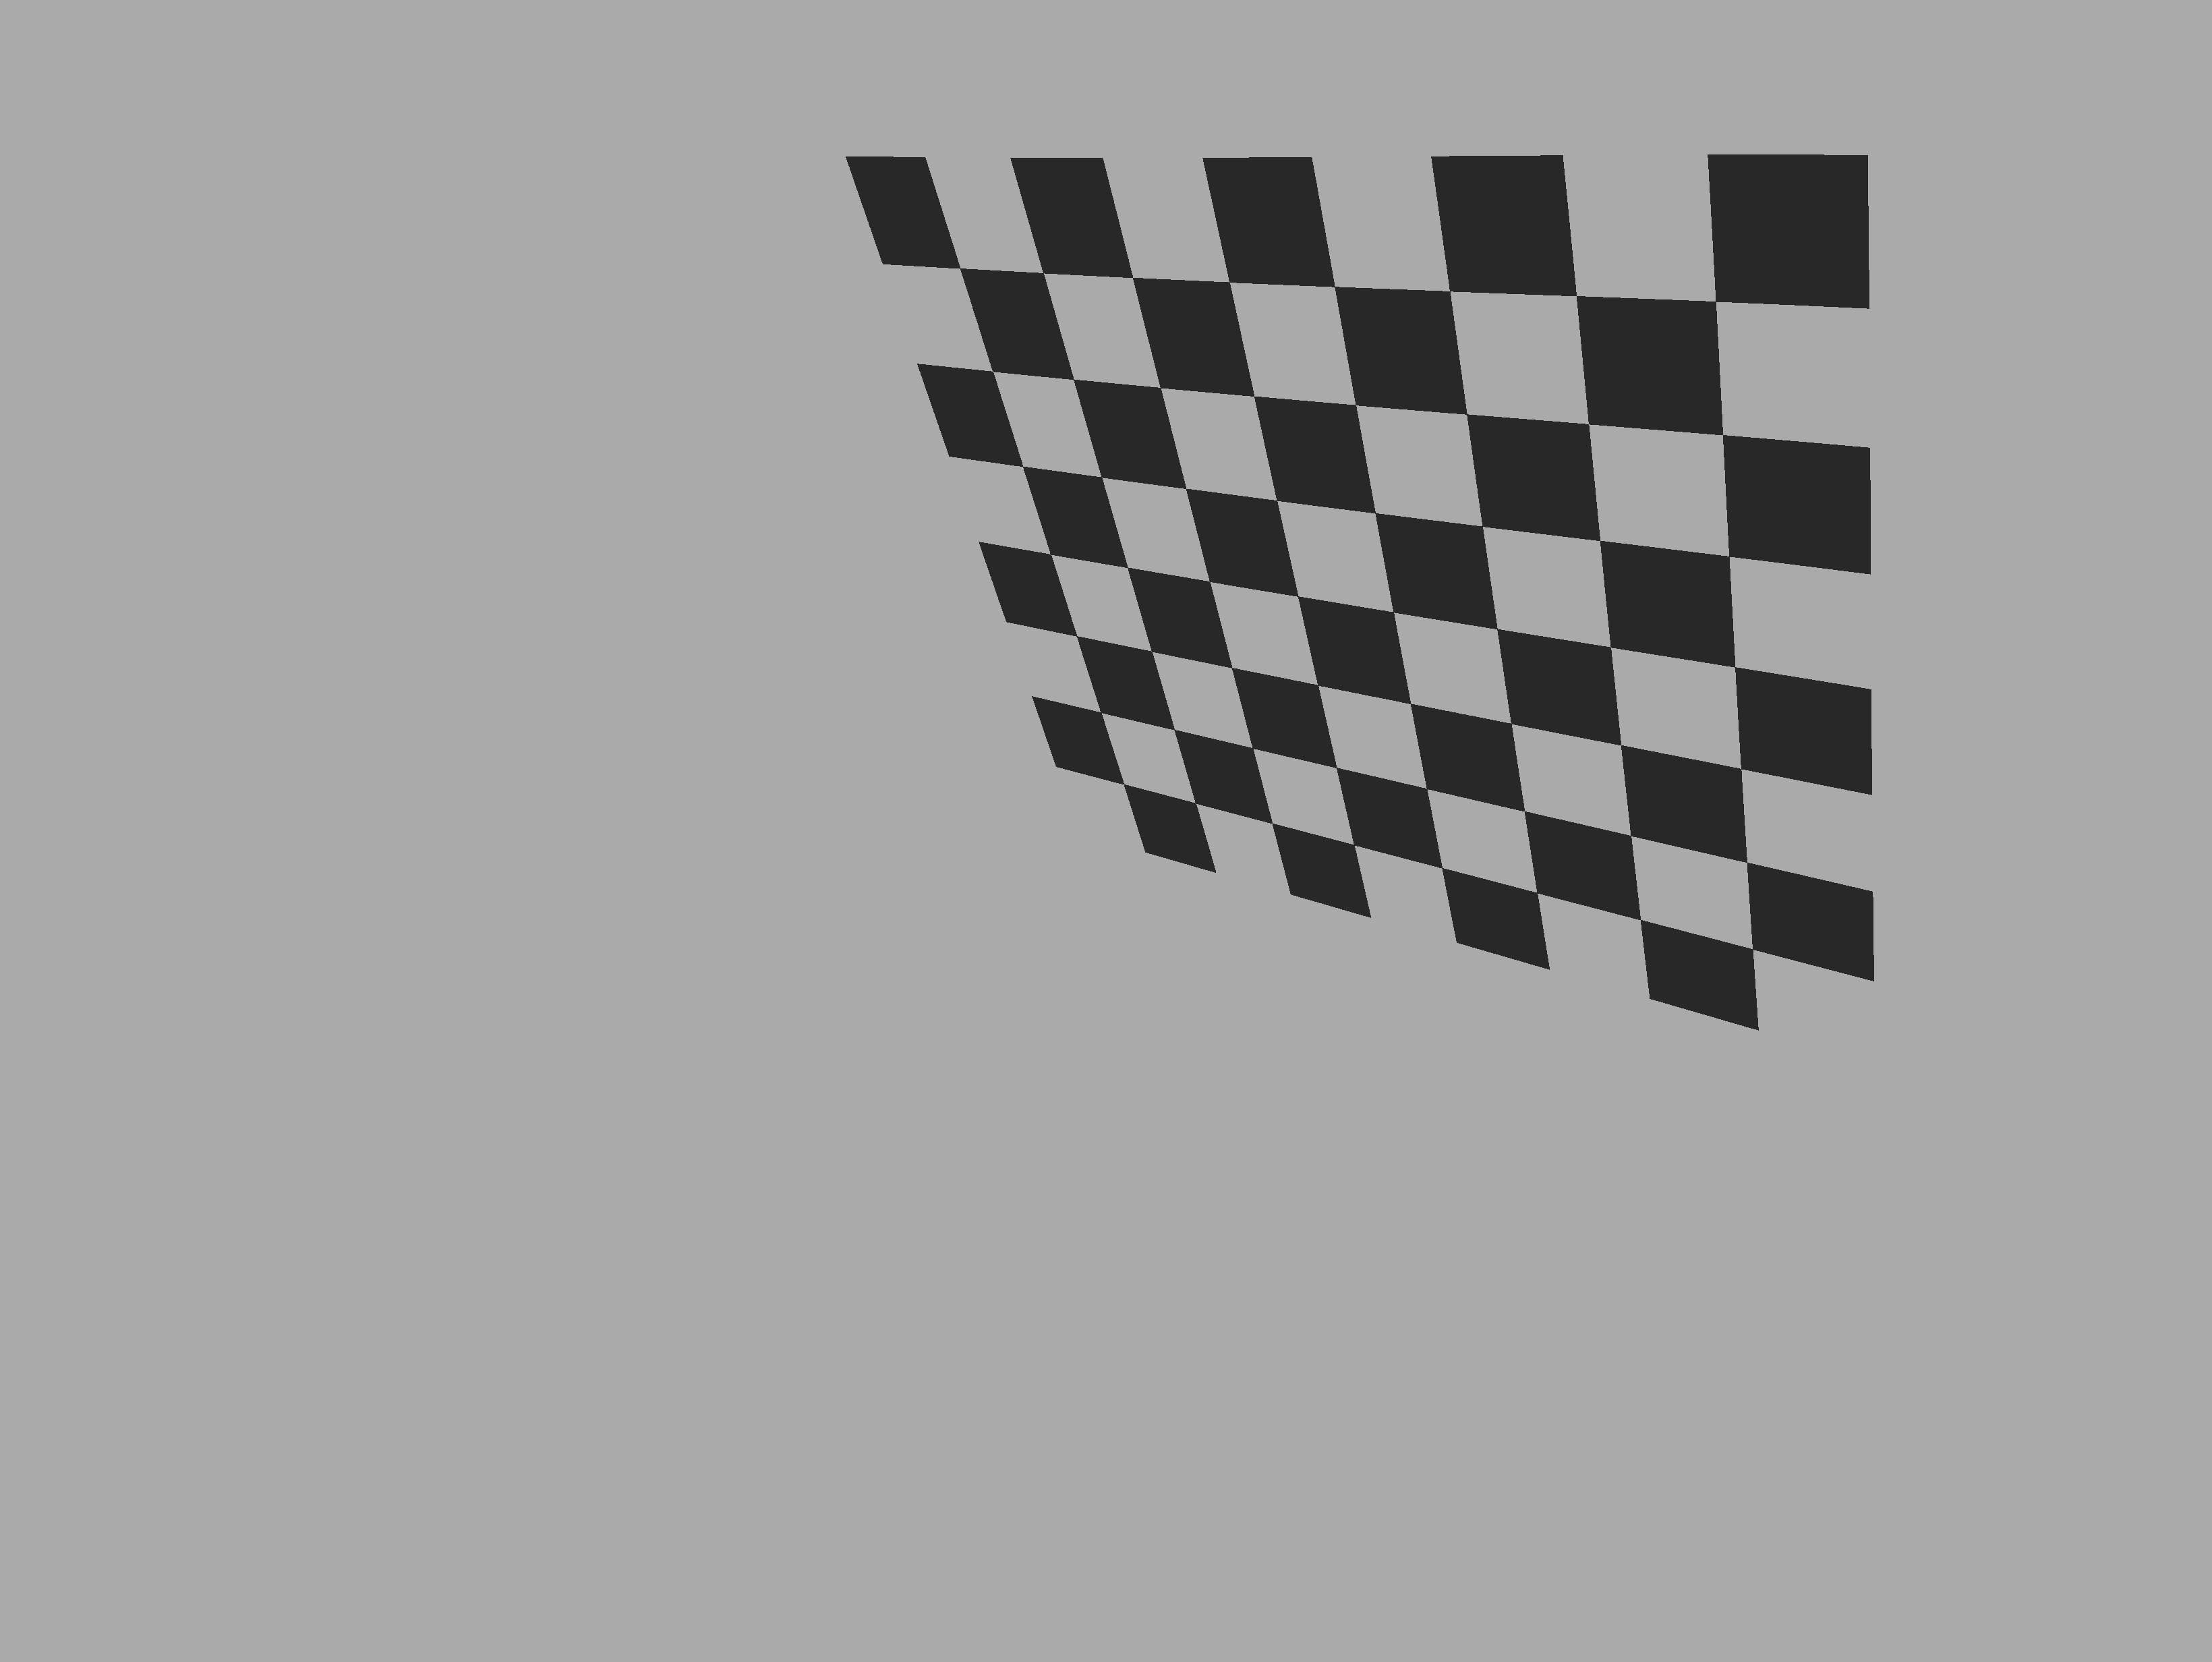
\includegraphics[width=0.3\linewidth]{3-development/calibration/images/im3.png}}
	\subfigure[\label{development:im4}]{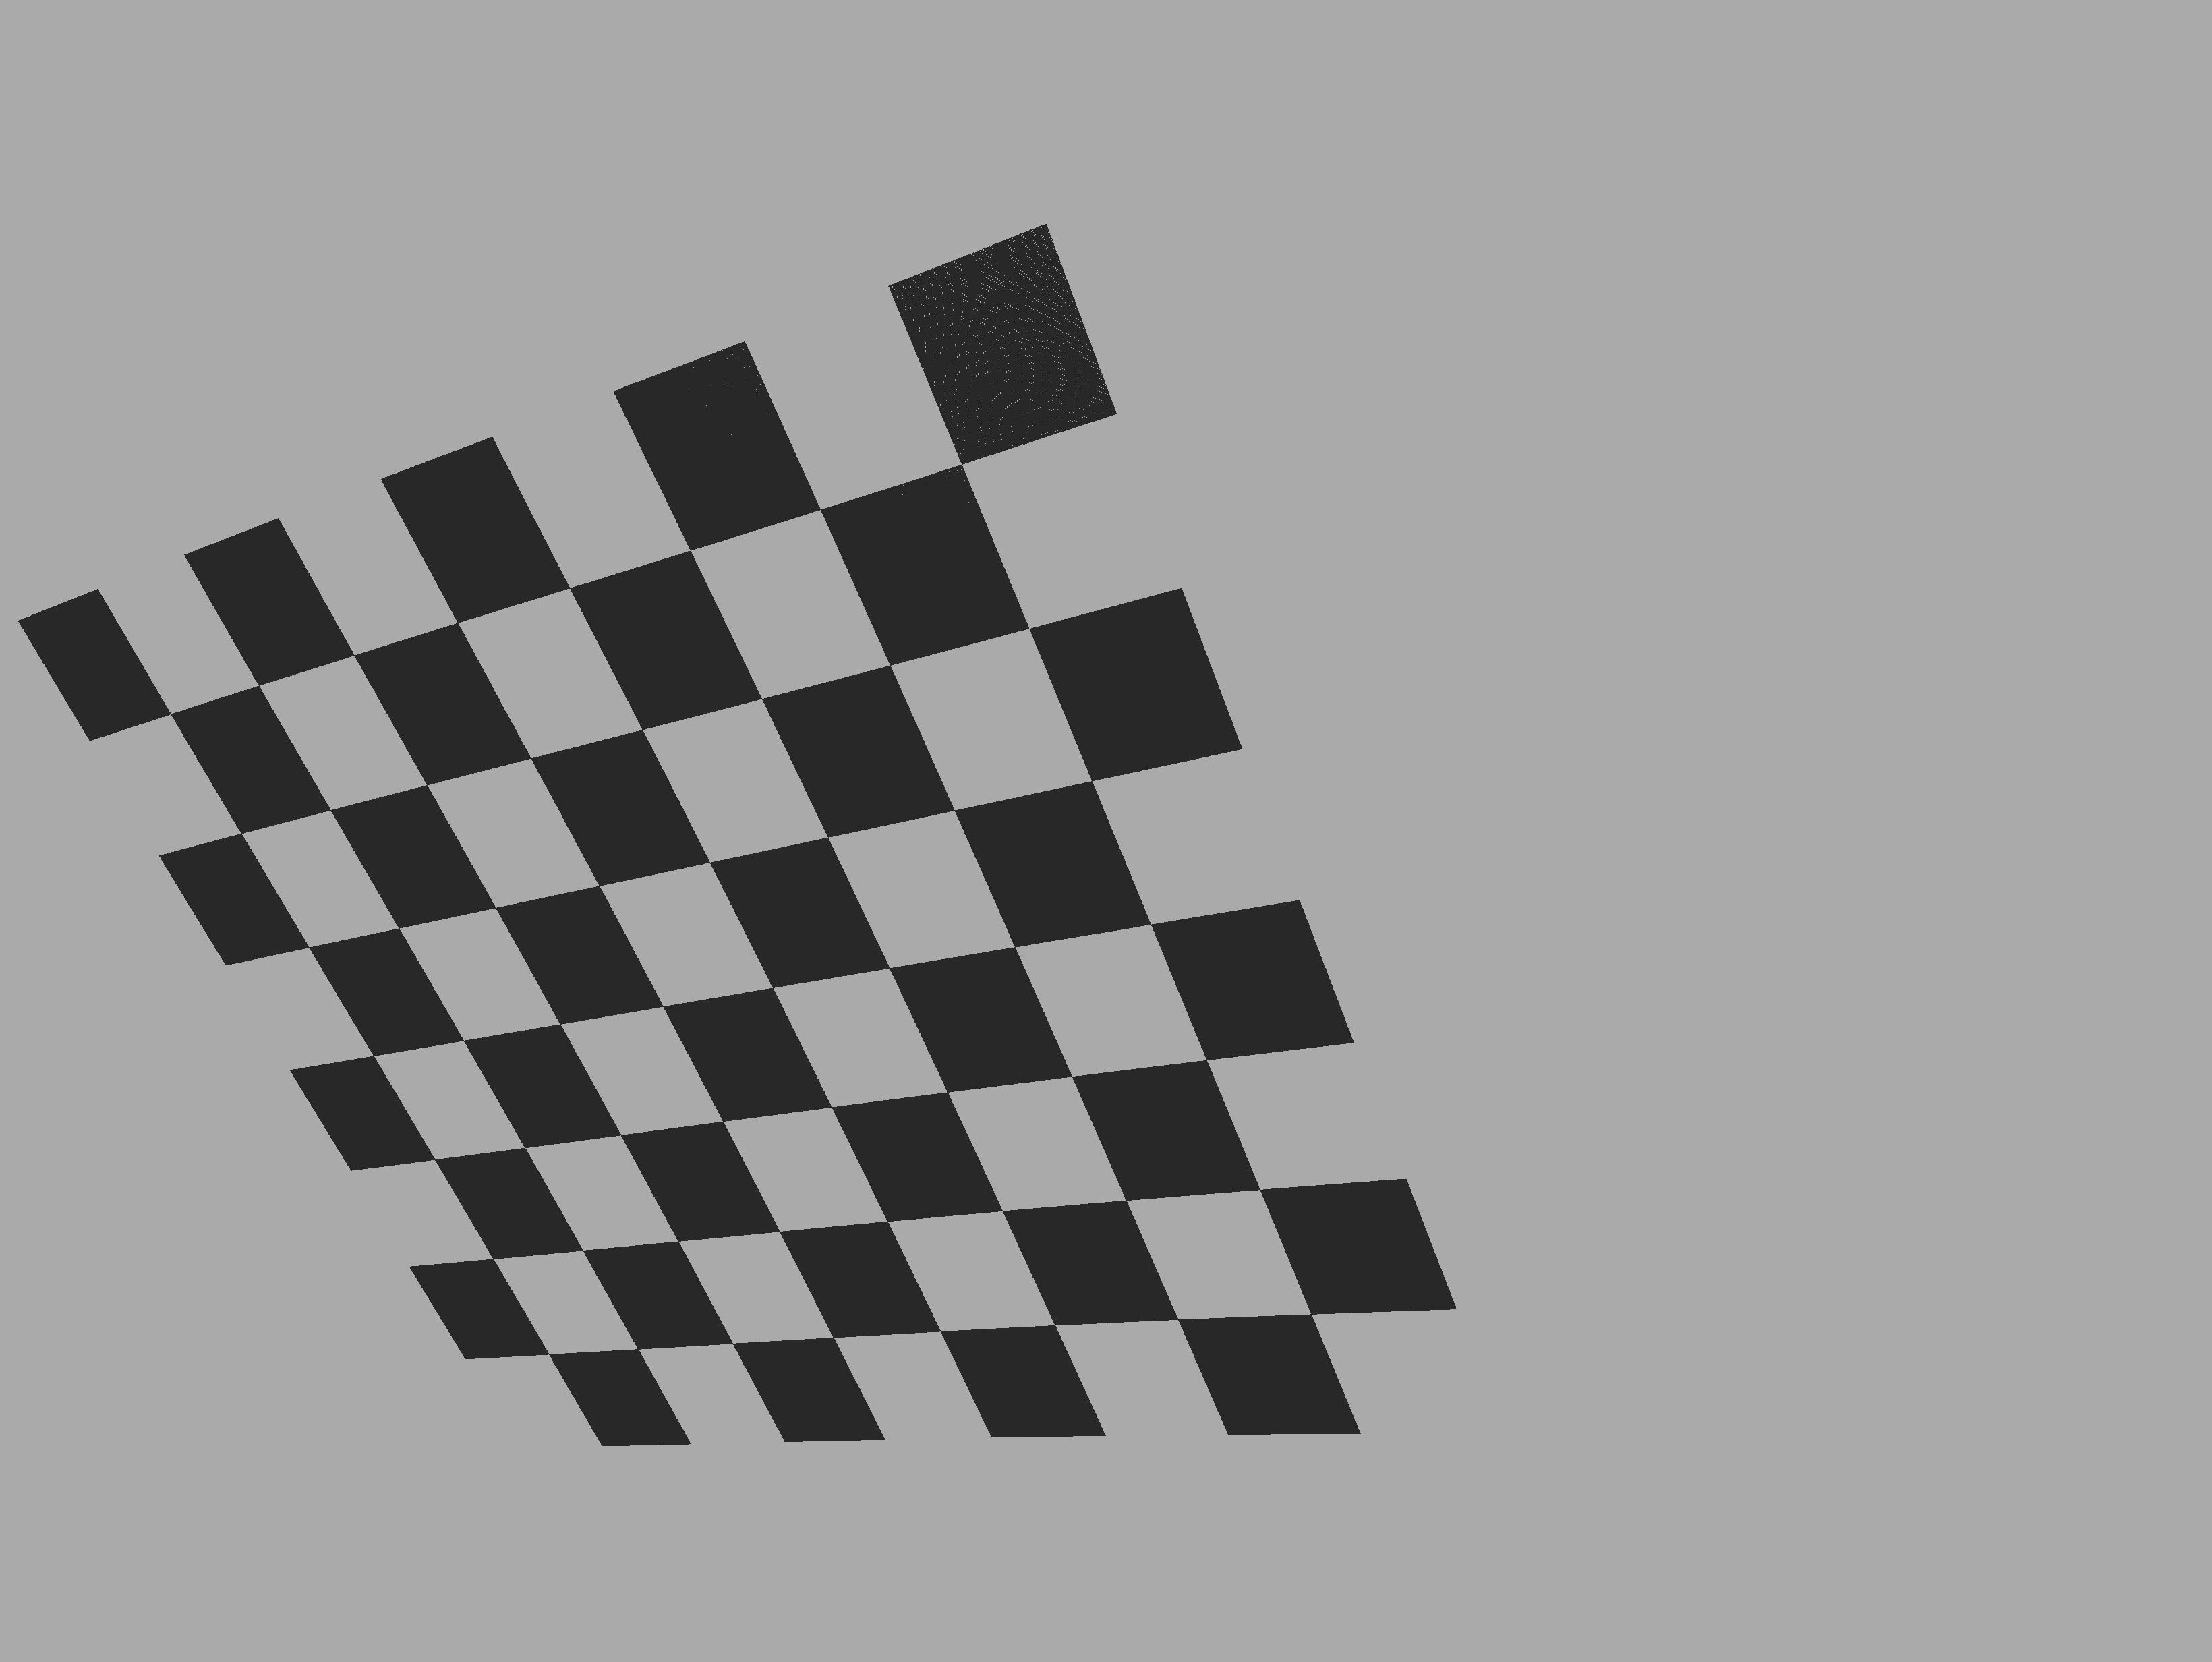
\includegraphics[width=0.3\linewidth]{3-development/calibration/images/im4.png}}
	\subfigure[\label{development:im5}]{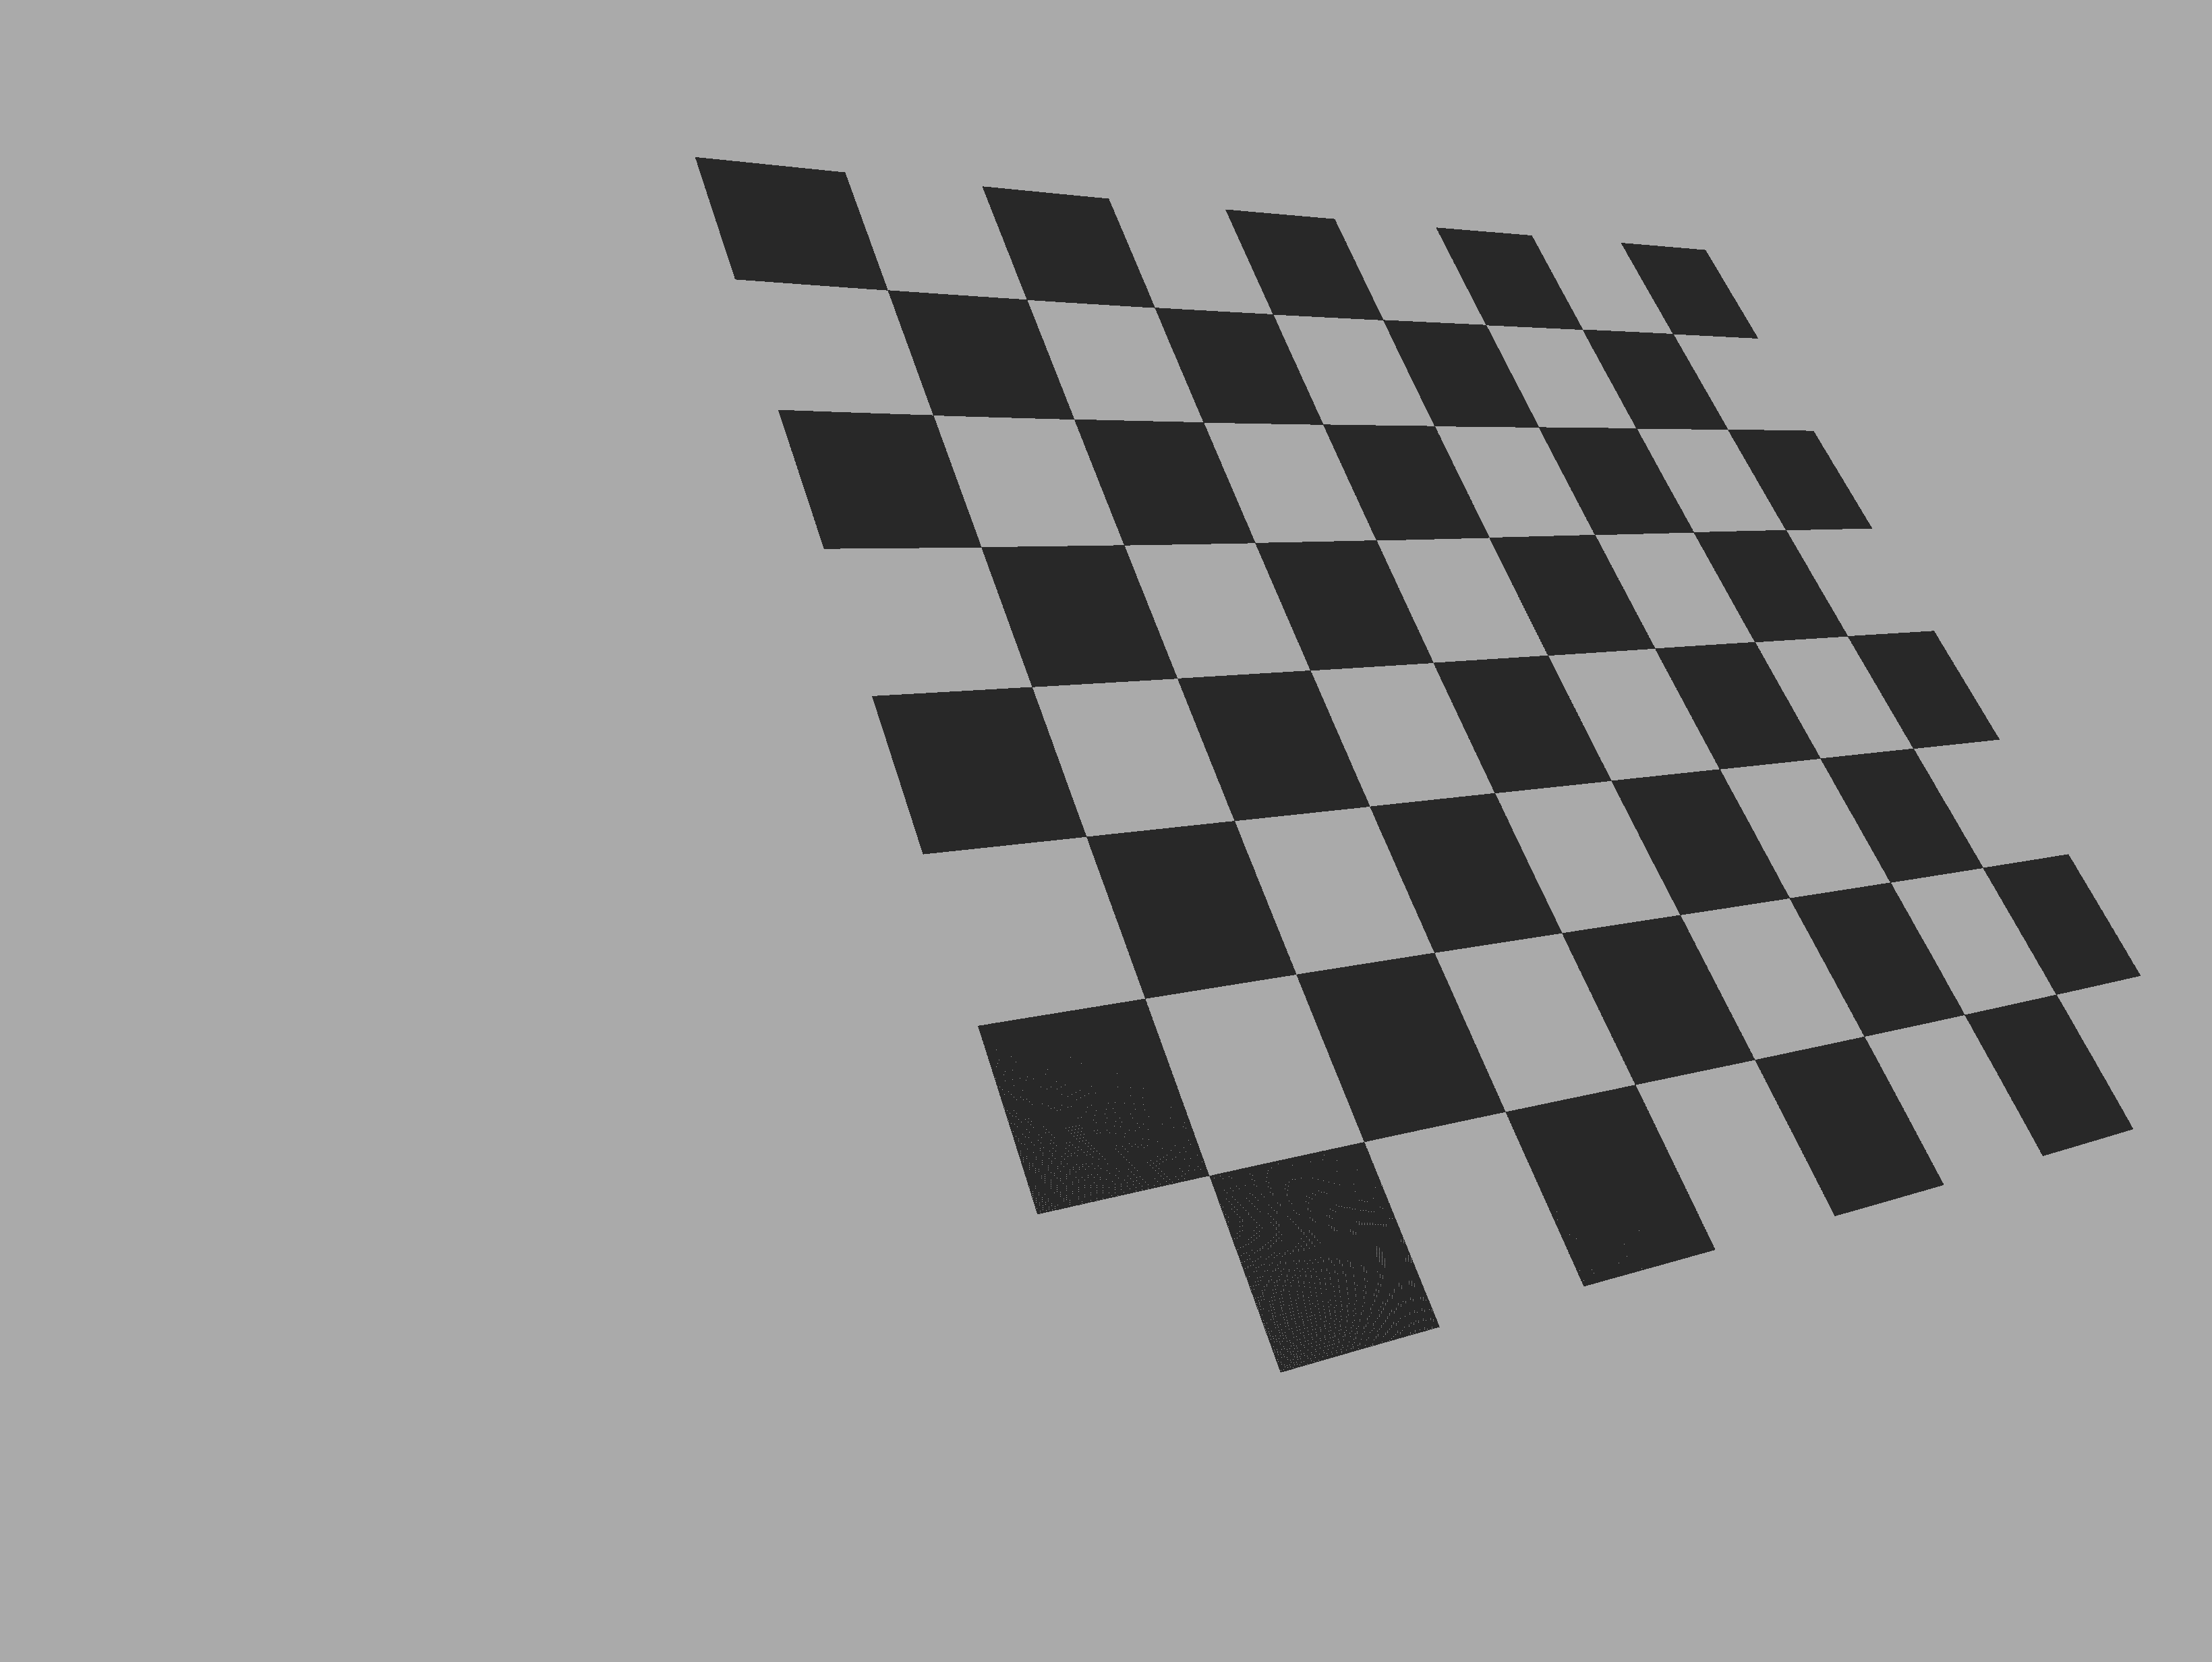
\includegraphics[width=0.3\linewidth]{3-development/calibration/images/im5.png}}
	\caption{Some of the 200 images \label{development:im}}		
\end{figure}

Randomly selected from these 200 are ten sets of each 20 images.
Now, the camera is calibrated separately with each set.
To visualize the result, the difference from the (with the model in equation \ref{theory:dist}) distorted and undistorted pixel-position is plotted. 
And this on all locations of half the diagonal in the upper right quadrant of the image.
In other words, we take a look at the distortion between the image center and the upper right corner where the minimal $r_{\text{min}}=0$, respectively the image center and the maximal radius $r_{\text{max}}=2051$ which of course depends on the image resolution.

This plot is shown in Figure \ref{development:stat}.
Each label displays the reprojection error.
The problems which occurred in the first attempts are clearly visible in the scattering of the curves.

\begin{figure}[ht]
	\centering
	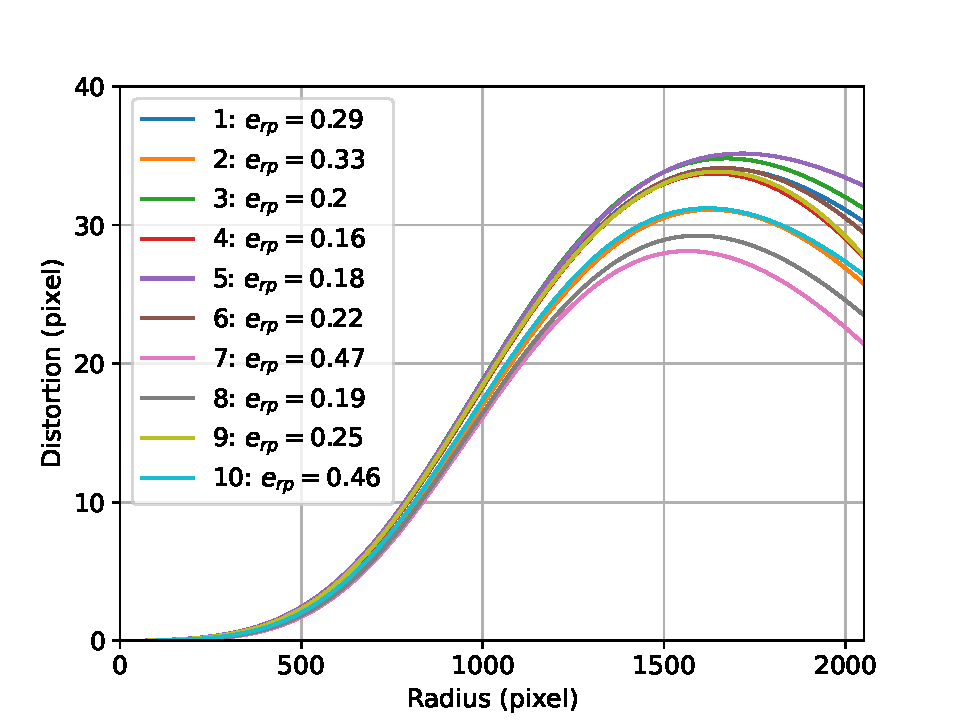
\includegraphics[width=0.9\linewidth]{3-development/calibration/images/stat.pdf}
	\caption{Distortion over the radius according to different sets if images\label{development:stat}}
\end{figure}

The distortion model introduces decentering effects and one could argue, that this plot should be made in all quadrants of the image.
But since the decentering effects are rather small in comparison with the radial distortion which is symmetric with respect to the centerpoint, it should be sufficient to plot only one quadrant.
Thus the assumption is made, that if the distortions are high in one quadrant, that the distortions in all other quadrants is also high and vice versa.

\subsection{Numpy-checkerboards\label{development:checker}}  
To estimate the contribution to the bad result of for example additive noise or blurred edges, one has the observe each effect isolated.

In order to do that, a python script was written, which generates a checkerboard as a numpy-array.
This array is then translated and rotated in three dimensions, and projected back to the 2D-plane.
As a last step, the images is distorted by the model in \ref{theory:dist} with the coefficients set to:
\begin{center}
	\begin{tabular}{lll}
		$k_1 = 4.1$   &$k_2 = 36$     &$k_3 = 38$\\
		$k_4 = 4$     &$k_5 = 34$     &$k_6 = 40$\\
		$p_1 = 0.002$ &$p_2 = 0.0019$ &$s_1 = -0.0014$\\
		$s_2 = -0.001$&$s_3 = -0.0022$&$s_4 = 0.00013$	
	\end{tabular} 
\end{center}
These coefficients were not chosen randomly, but were taken from a calibration which was made with one of the ten sets from the calibration statistics in \ref{development:statistics}.
They should therefore not be completely off.
Some of these (in total 24) images are shown in Figure \ref{development:nump}
To stay close to the real camera, these are not black and white images.
The black part has a value of 40 and the white a value of 170.
The means of the images come with these values close to 127, which is the value which the exposure control of the camera aims to achieve.

\begin{figure}[ht]
	\centering
	\subfigure[\label{development:nump0}]{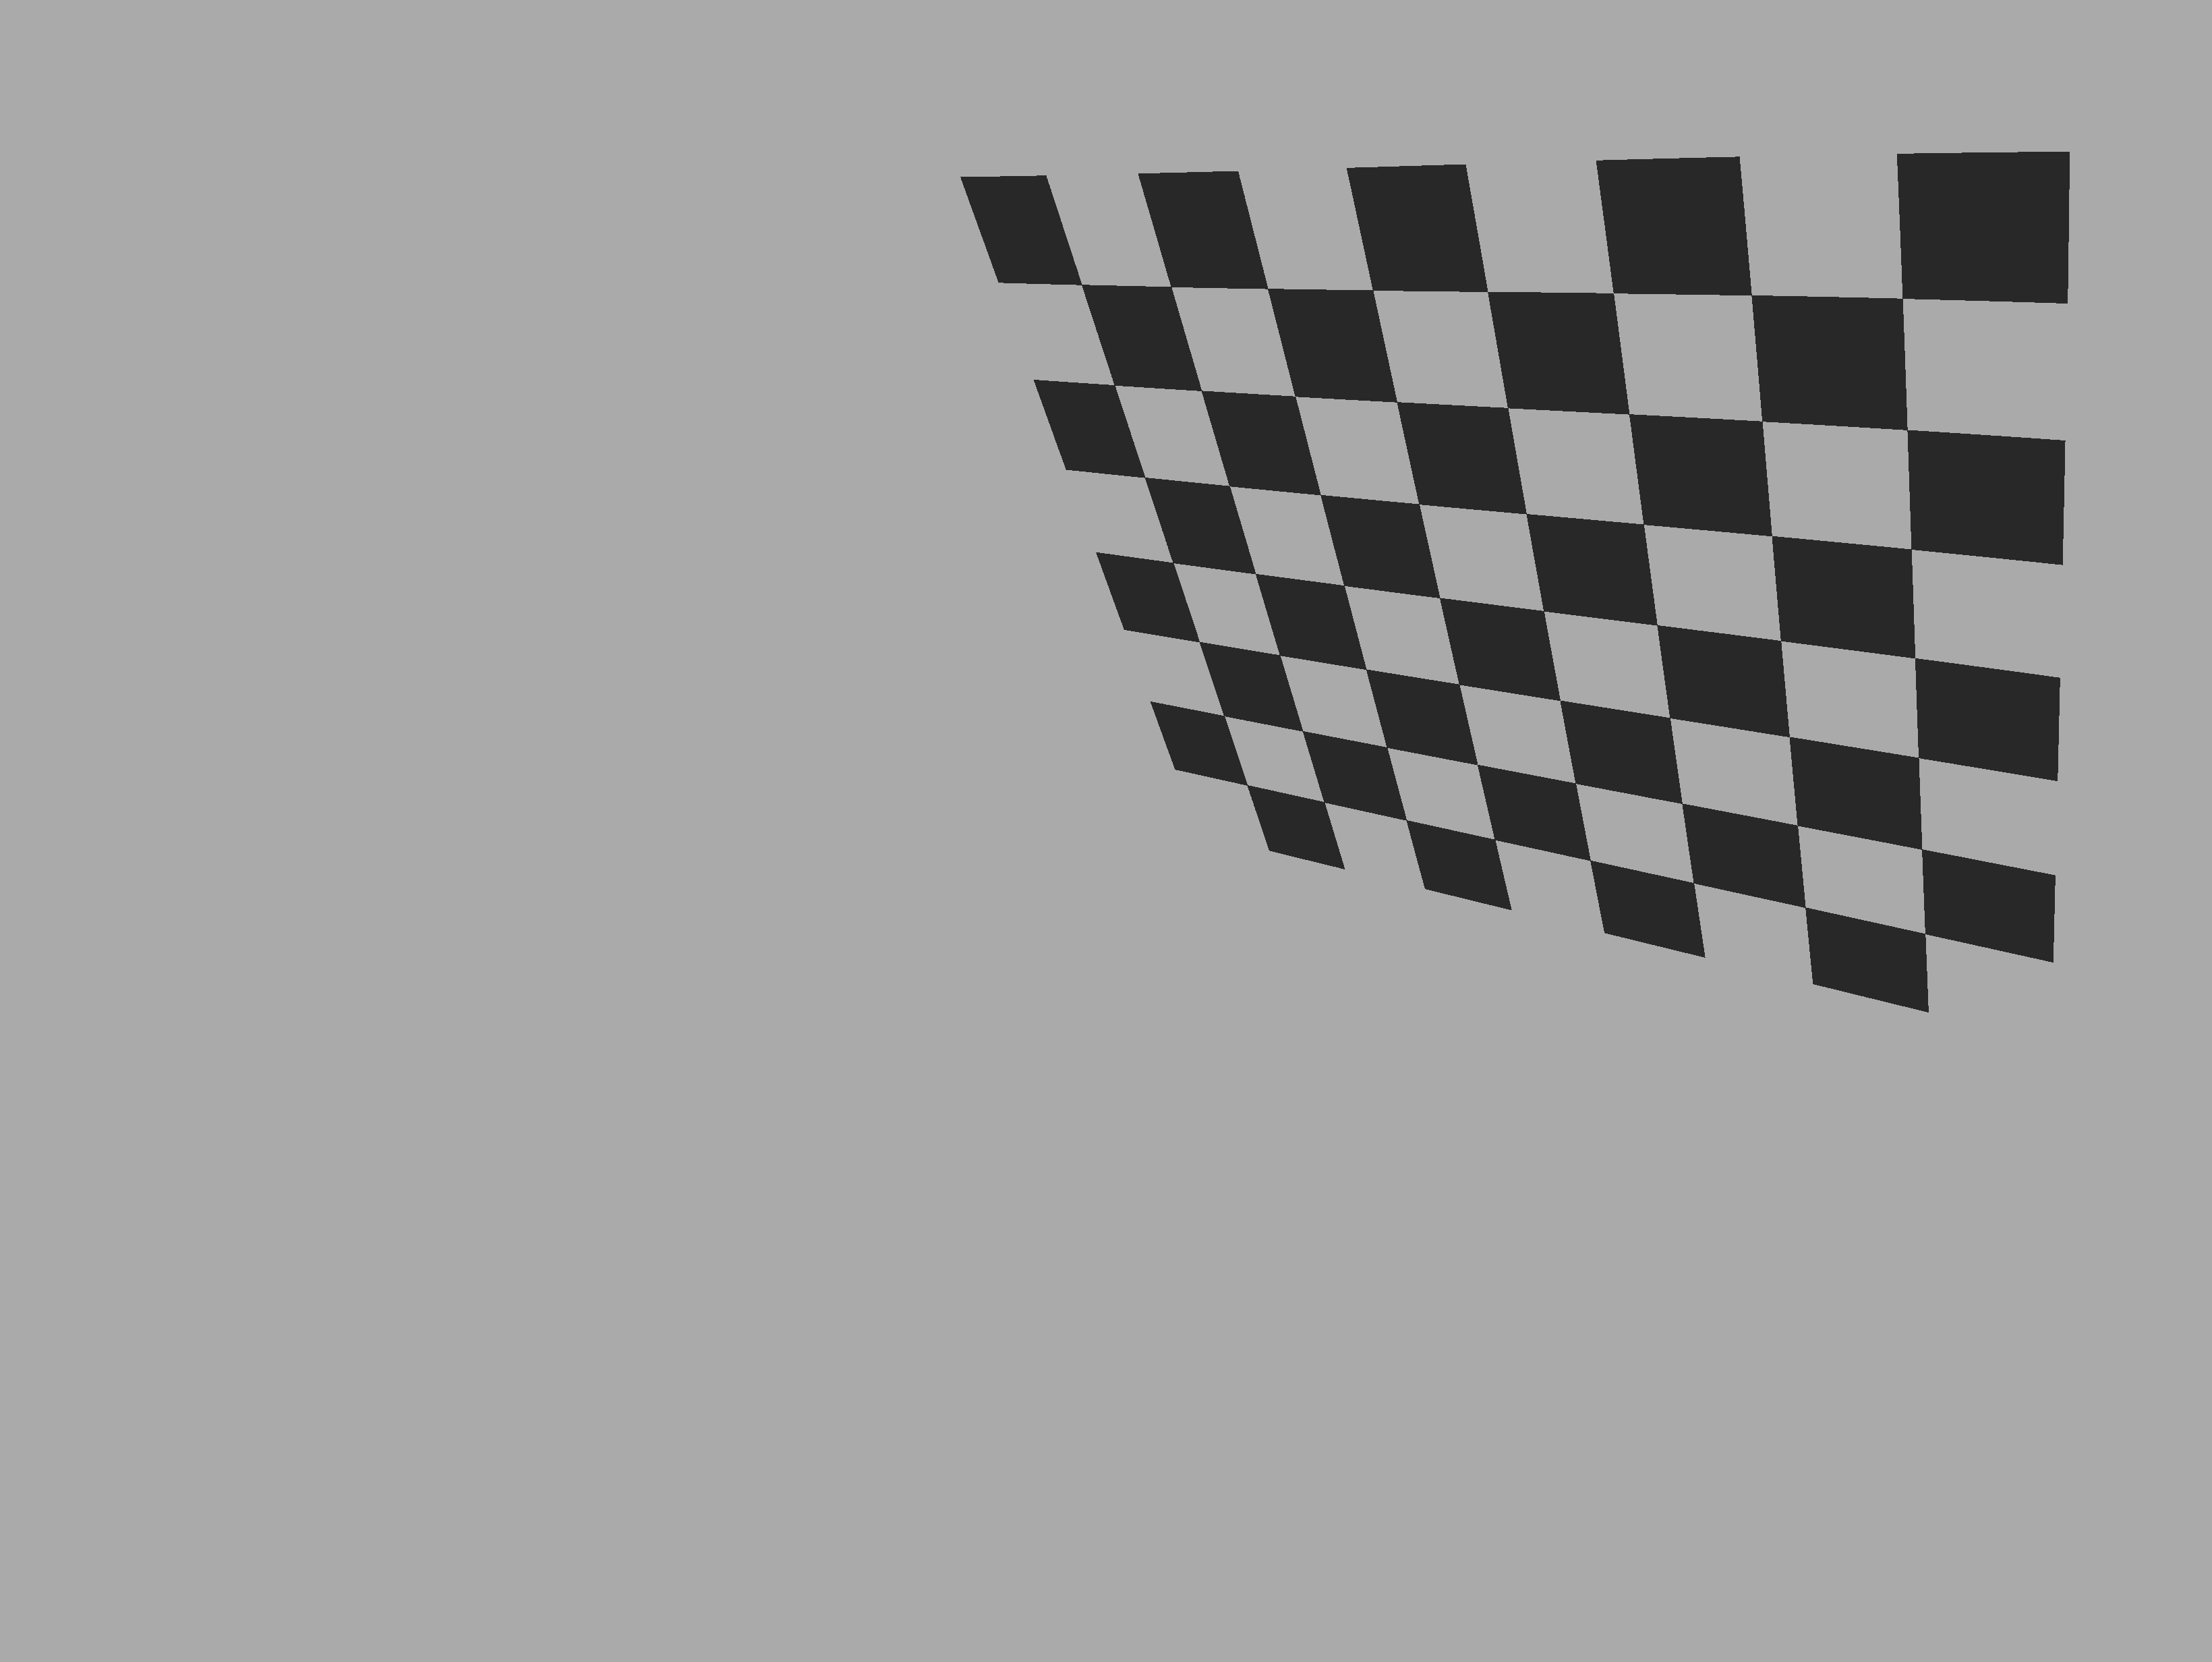
\includegraphics[width=0.3\linewidth]{3-development/calibration/images/nump0.png}}
	\subfigure[\label{development:nump1}]{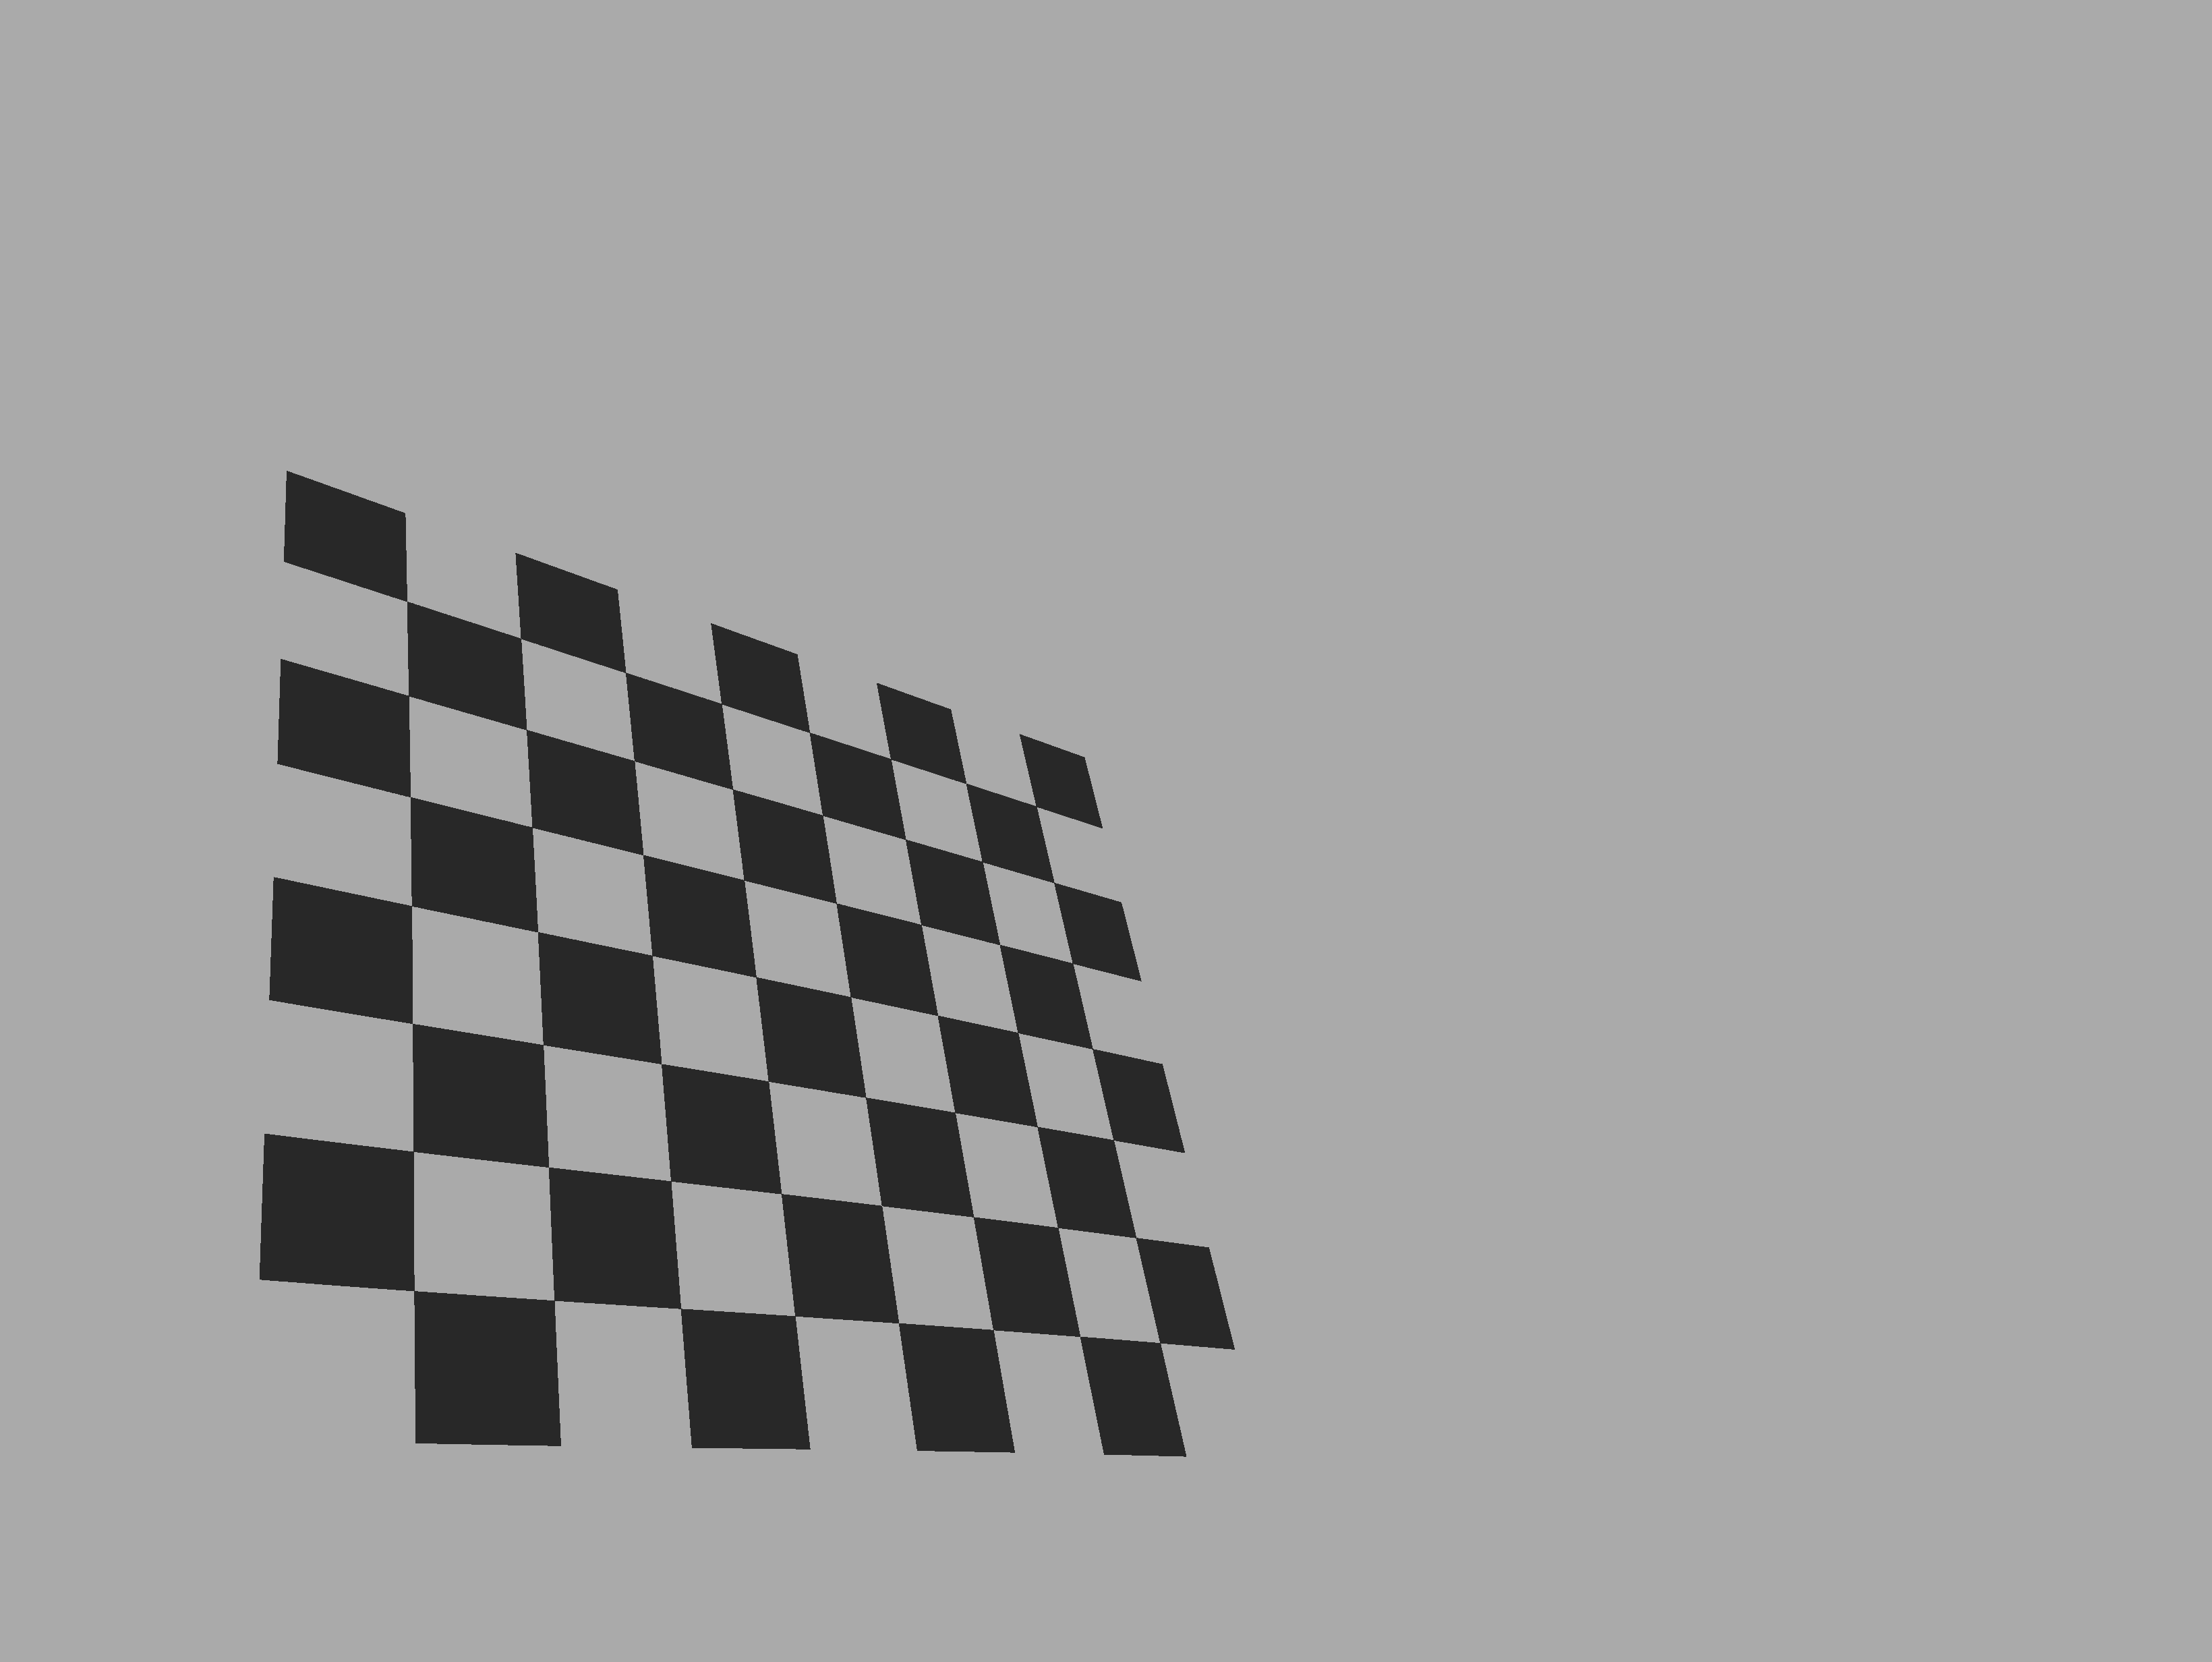
\includegraphics[width=0.3\linewidth]{3-development/calibration/images/nump1.png}}
	\subfigure[\label{development:nump2}]{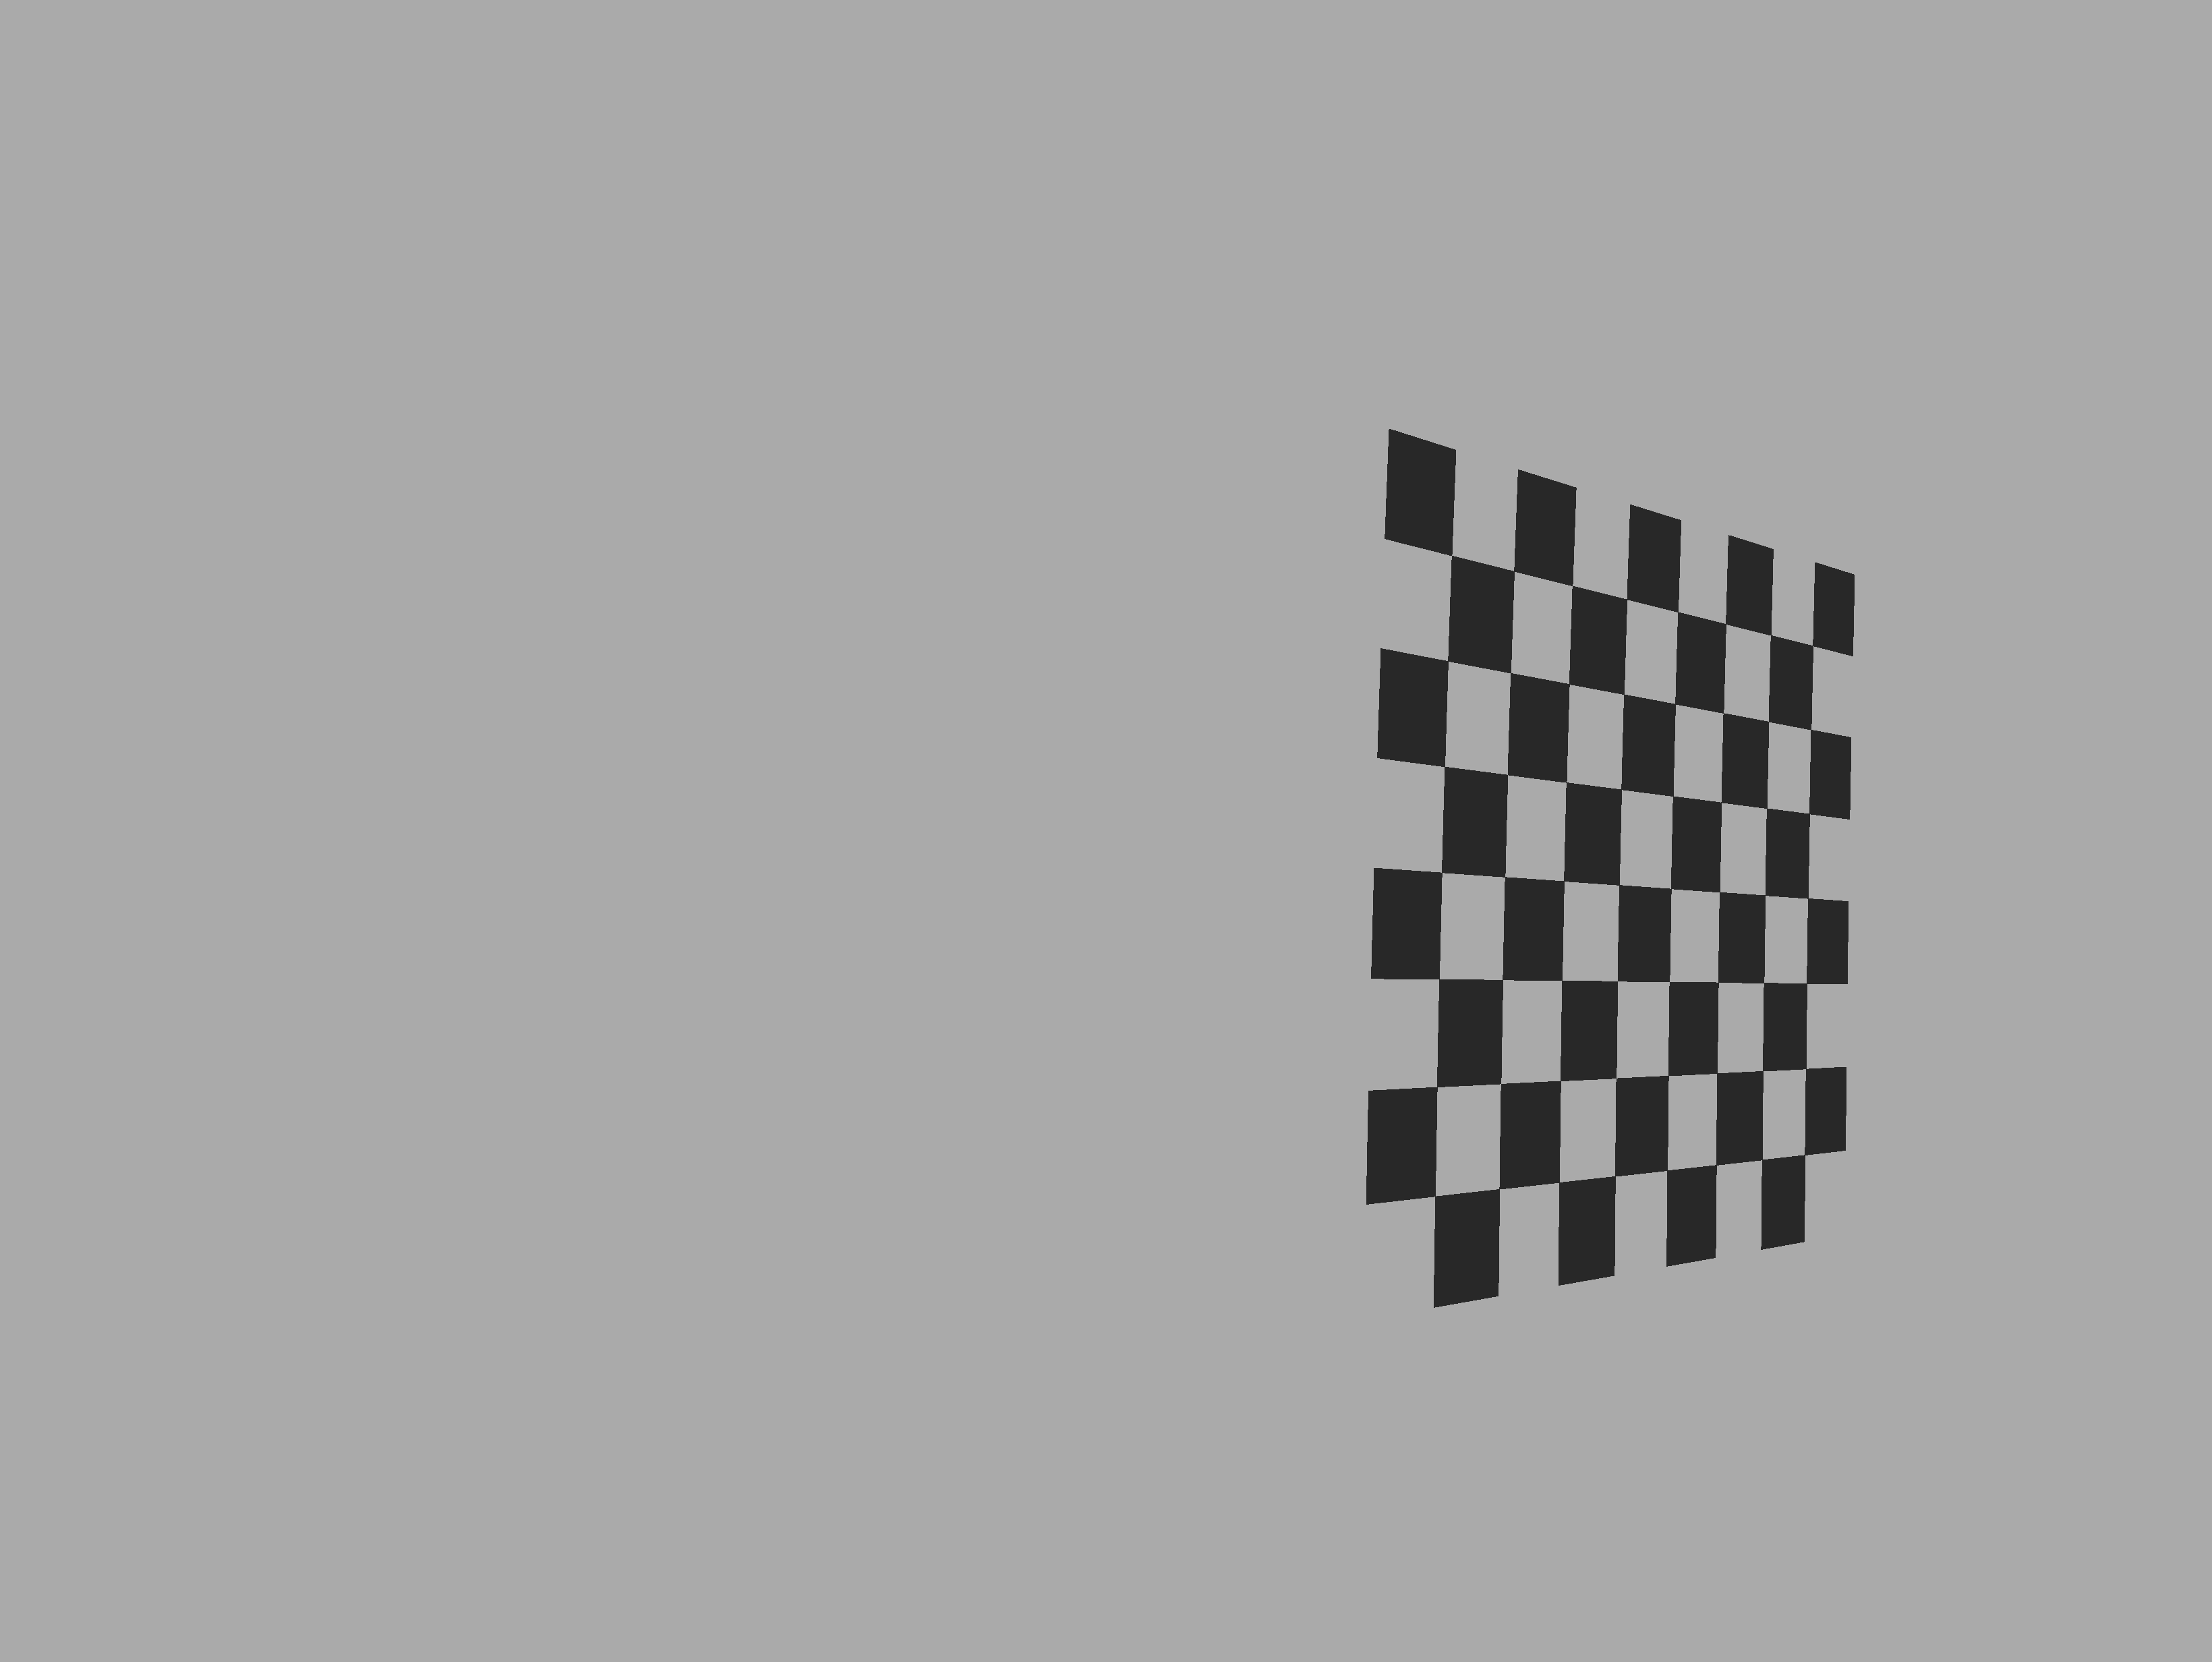
\includegraphics[width=0.3\linewidth]{3-development/calibration/images/nump2.png}}
	
	\subfigure[\label{development:nump3}]{
\includegraphics[width=0.3\linewidth]{3-development/calibration/images/nump3.png}}
	\subfigure[\label{development:nump4}]{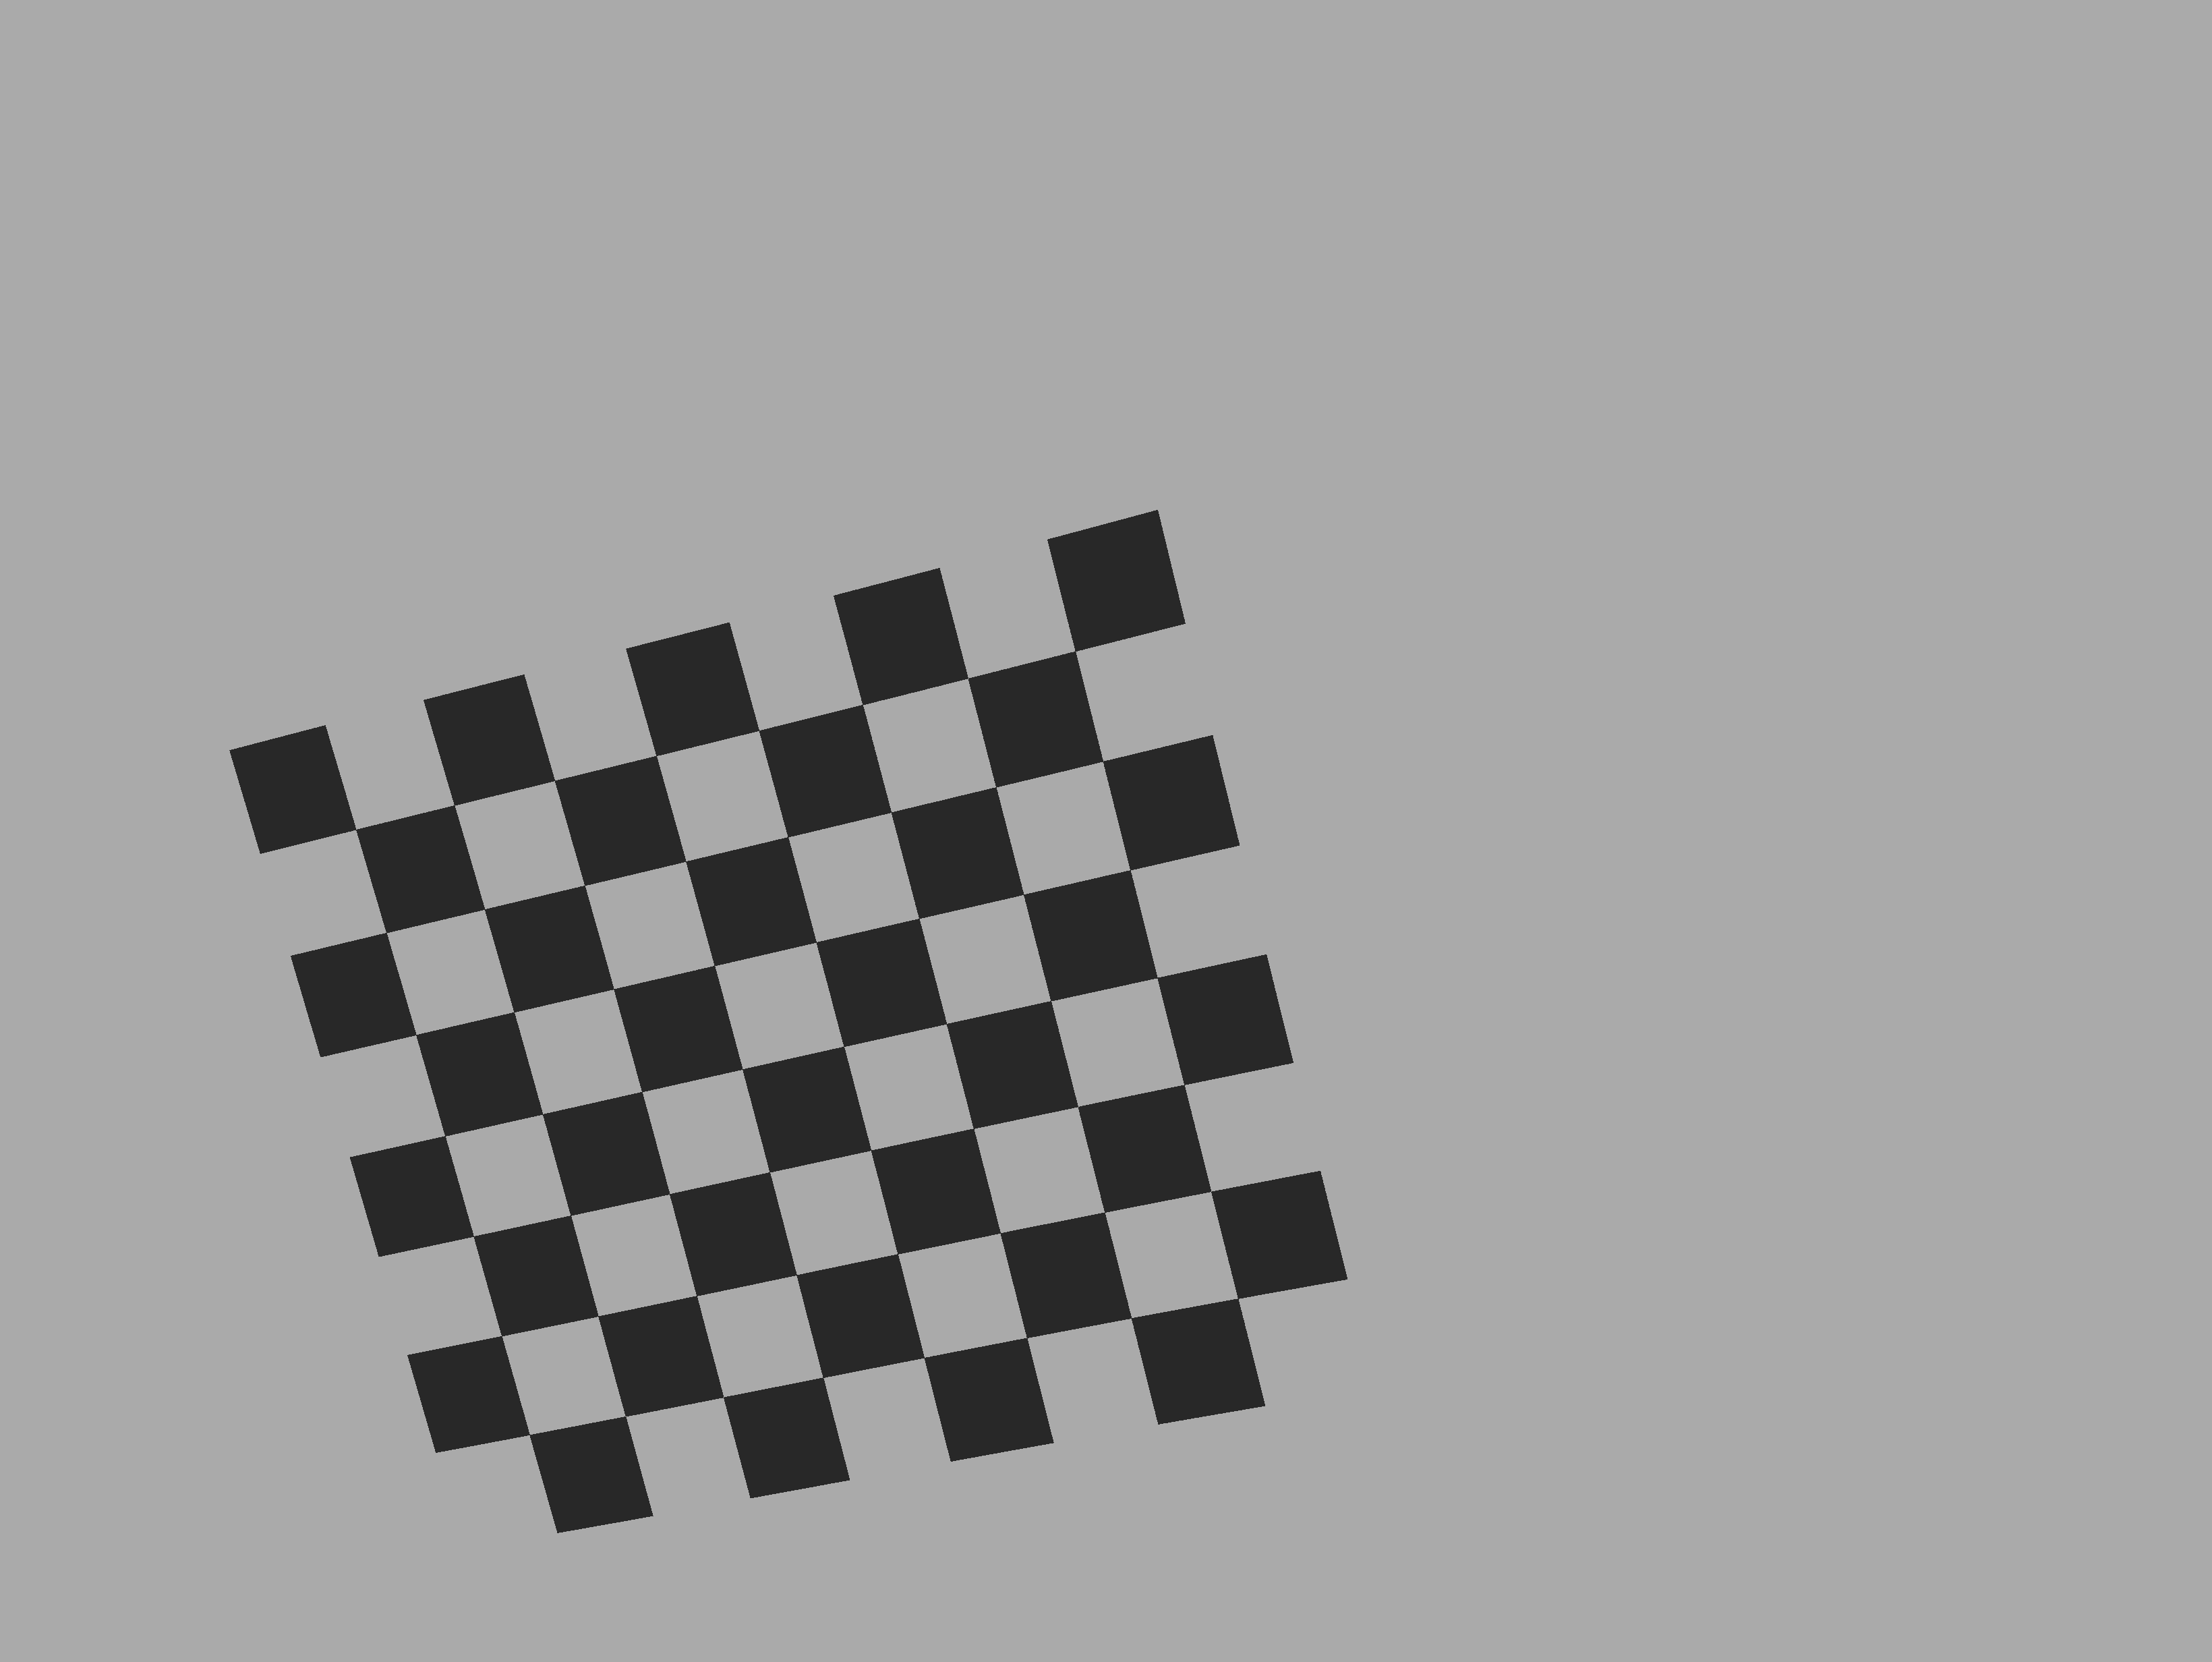
\includegraphics[width=0.3\linewidth]{3-development/calibration/images/nump4.png}}
	\subfigure[\label{development:nump5}]{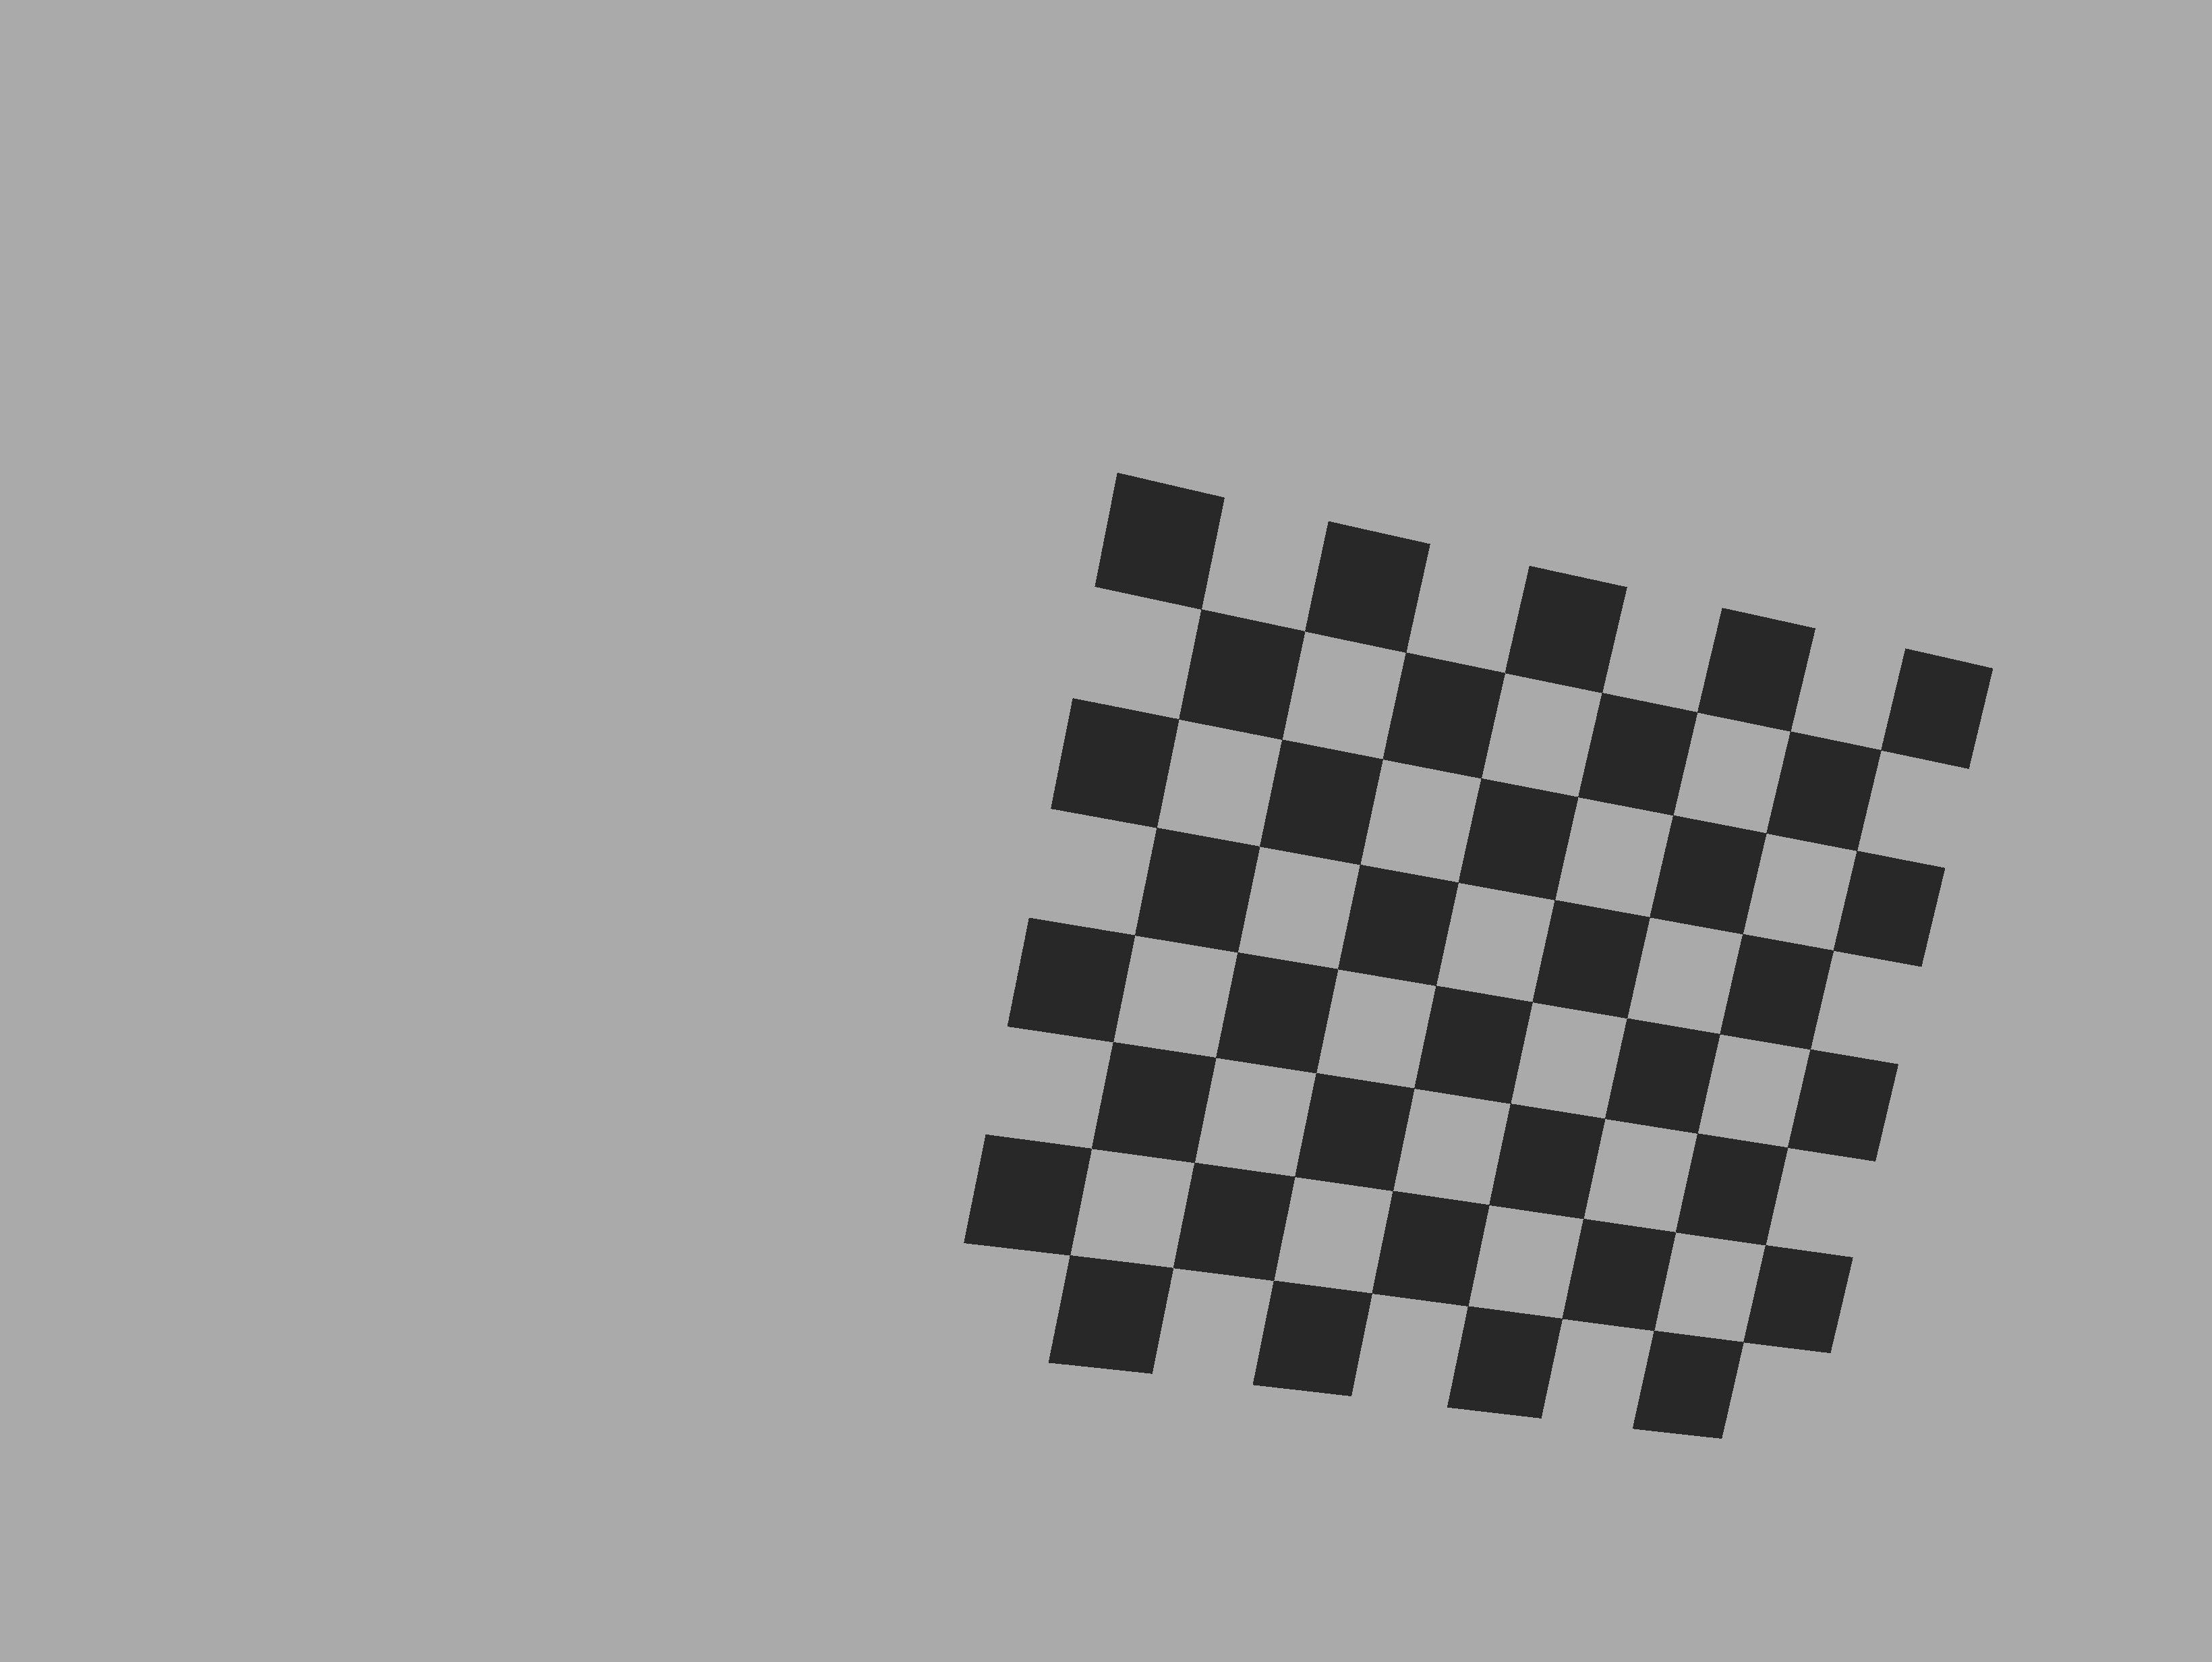
\includegraphics[width=0.3\linewidth]{3-development/calibration/images/nump5.png}}
	\caption{Some of the numpy-arrays \label{development:nump}}		
\end{figure}

These numpy-checkerboards can now be further manipulated to simulate real effects.
To asses, how much these effects influence the calibration, the coefficients obtained by the calibration process can be compared to the real coefficients which were used to distort the images in the first place.

\subsection{Possible cause of errors}
This subsection takes a closer look on details, which could be influencing the calibration and lead to the bad results in section \ref{development:statistics}.
The numpy-checkerboards where hereby used as a basis.

\subsubsection{Location of the checkerboard in the image}
To show that it is important to include images in the calibration process, in which the checkerboard has corners very close to the image corners, the calibration has been performed two times.
The first did include images like \ref{development:nump0} - \ref{development:nump4} and similar, but not images, where the checkerboard reached outside the frame, like \ref{development:nump5}.
The second calibration included all images.

Again a plot of the distortion, as described in section \ref{development:statistics} is generated.
This plot shown in Figure \ref{development:loc}, contains the real model coefficients and the ones, which were obtained by the calibration.
The label displays additionally the reprojection error.
\begin{figure}
	\centering
	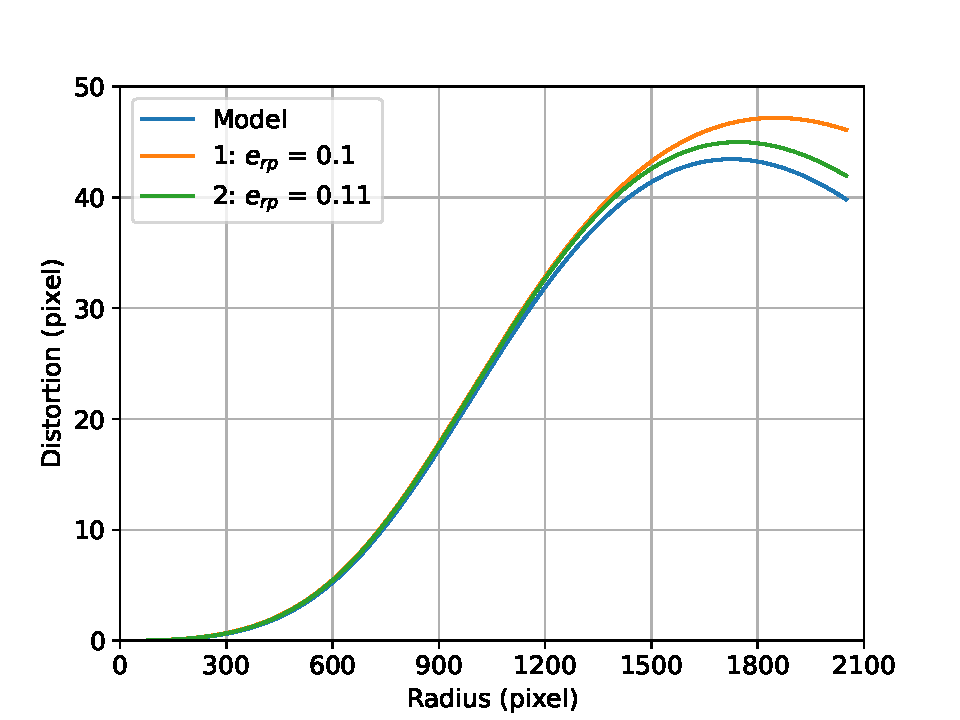
\includegraphics[width=0.9\linewidth]{3-development/calibration/images/location.pdf}
	\caption{Comparison of the calibration to the model. 1: Excluding images with checkerboards overlapping the frame, 2: All images included \label{development:loc}}
\end{figure}
There is no discussion that the second calibration (including all images) does a much better job and follows the real curve closer.
At the maximal radius, the difference between the model and the second calibration is 2.12 pixel.
This also illustrates, that the reprojection error is really a training error rate and is not sufficient to asses the quality of the calibration.

One further observation can be made: The second calibration represents some sort of best case calibration.
The only error comes from the detection of the checkerboard corners and since these numpy-checkerboards have the sharpest possible edges and there is no noise in the image, it is impossible detect the corners more precise in a real environment with these methods.
Thus to get a better calibration, a better feature detection is necessary and its development would take more steps into account which are not in the scope of this thesis.

\subsubsection{Additive noise in the image} 
Exposure in photography contains of three parts: aperture, shutter speed and ISO (light sensitivity).
The camera operates in automatic exposure control and tries to fix the average brightness to 127.
Since the aperture is fixed, it can only adjust the shutter speed and ISO.
If the overall environment is dark, the control needs to make the chip more sensitive against the incoming light by increasing the ISO.
This introduces noise into each image.

To get more insight on the properties of the noise, an image of a white background was taken.
The histogram of this image with a Gaussian fit is shown in Figure \ref{development:noise_dist}.
\begin{figure}
	\centering
	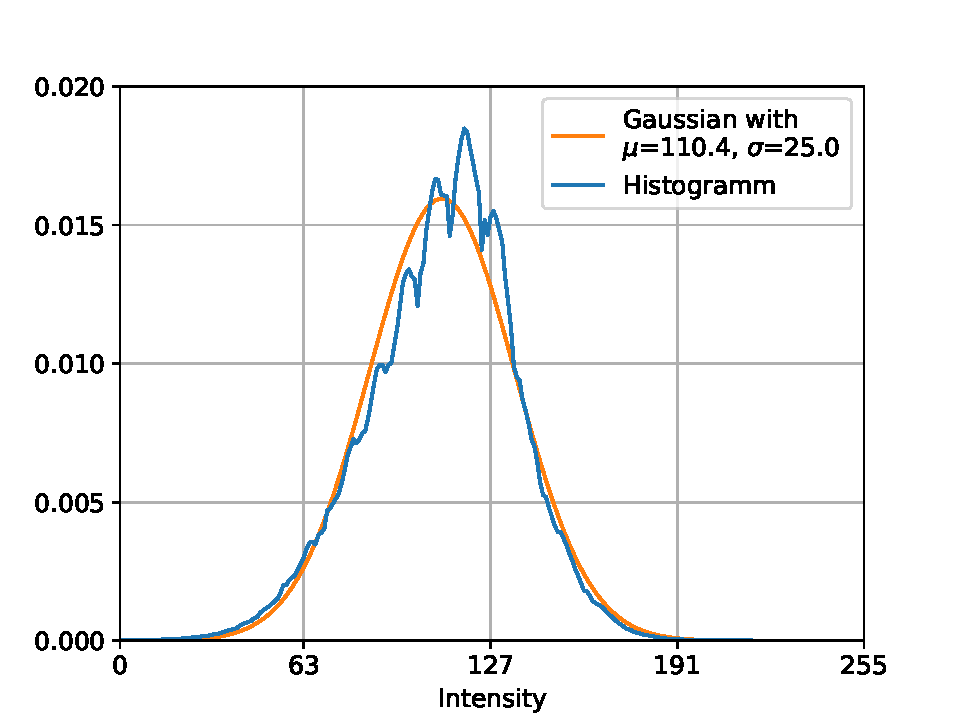
\includegraphics[width=0.9\linewidth]{3-development/calibration/images/noise_distribution.pdf}
	\caption{Histogram of an uniform white background with an Gaussian fit\label{development:noise_dist}}
\end{figure}
Since the background itself is (approximately) uniformly white, there should theoretically only be one spike at the intensity of 127 (fixed by the automatic exposure control).
But there is also noise introduced by the chip of the camera, which blurres the histogram.
As this plot shows, the assumption that the noise has a normal-distribution is, as one might expected, supported.

To understand now, how much this noise influences the calibration, zero mean additive white Gaussian noise with standard deviations from 0 to 50 (stepsize $=0.5$) is added onto each image and the calibration performed. 

It turns out, that more noise does not necessarily mean a worse calibration.
But there are some insights, which can be taken from this experiment.
Figure \ref{development:noise_rpe} shows how the reprojection error depends on the standard deviation of the additive white noise.
\begin{figure}
	\centering
	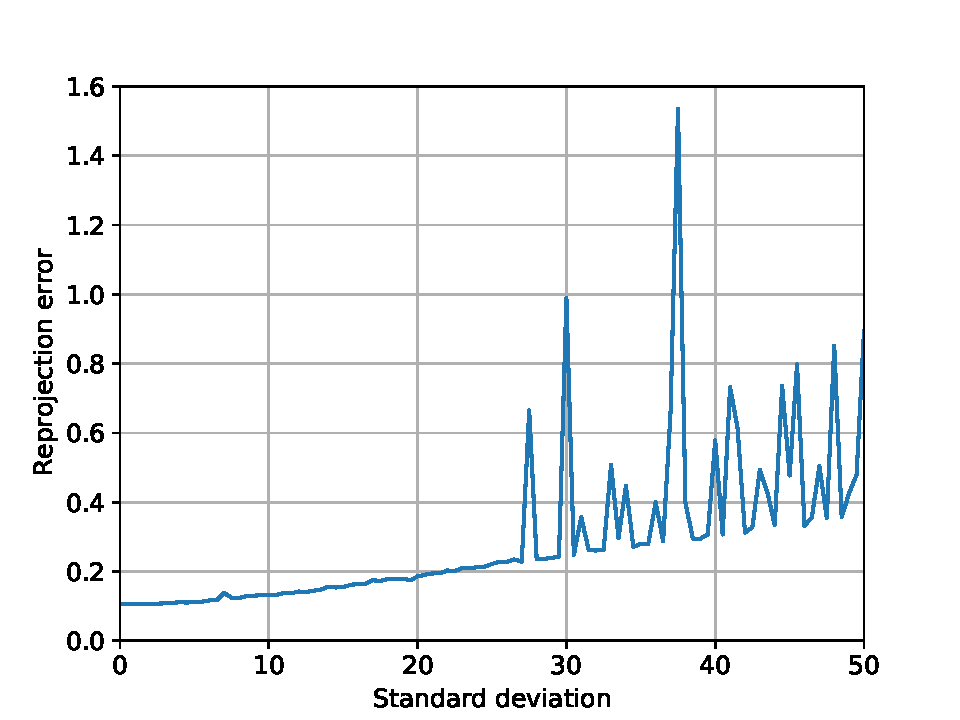
\includegraphics[width=0.9\linewidth]{3-development/calibration/images/noise_rpe.pdf}
	\caption{Reprojection error in dependence of additive noise\label{development:noise_rpe}}
\end{figure}
It was to be expected, that the reprojection error increases with more noise, but what really could pose a problem are the spikes.
It seems, that after a standard deviation of 25, bad reprojection errors become more likely even if the underlying increase is linear.

This can also be seen in Figure \ref{development:noise_k} where the radial coefficients are plotted.
Tangential and thin prism coefficients are not shown, since they show similar plots.
\begin{figure}
	\centering
	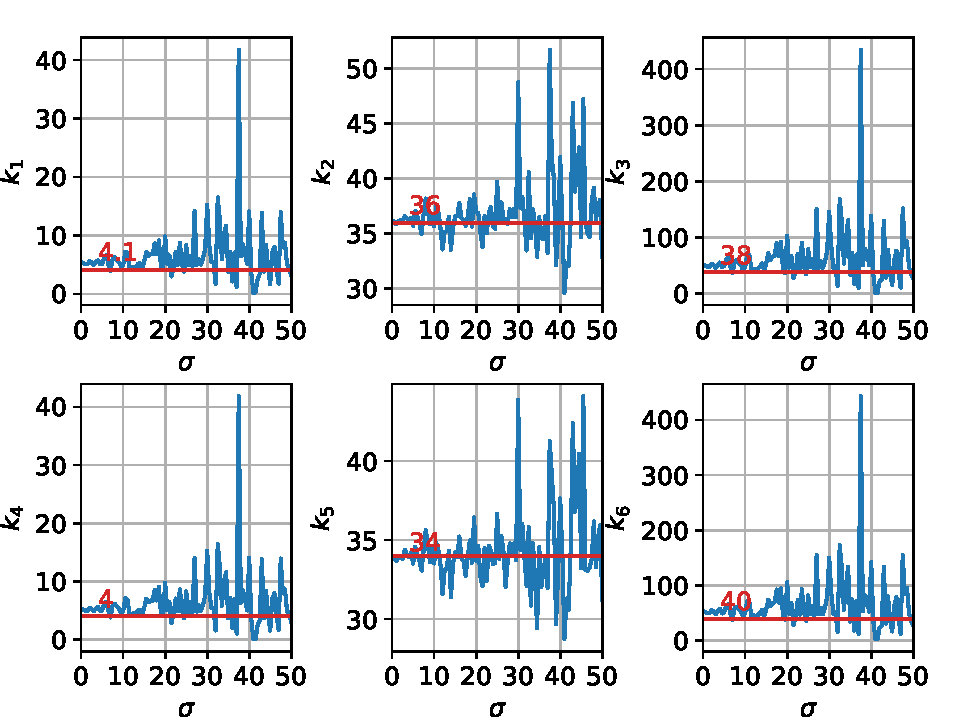
\includegraphics[width=0.9\linewidth]{3-development/calibration/images/noise_k.pdf}
	\caption{Blue: Calibrated radial coefficients in dependence of additive noise (deviation = $\sigma$). Red: Real coefficient\label{development:noise_k}}
\end{figure}
Again it seems that the calibration is not very reliable after a standard deviation of 25.
One can conclude, that noise does not affect the calibration directly, but can lead to unreliable results.
thus it is necessary to keep noise as low as possible .
this can be done by letting enough light reach the camera sensor, that the exposure control can keep the light sensitivity (ISO) low.

\subsubsection{Blurred images}
To get a grasp how the sharpness of each image affect the calibration, the numpy-checkerboards where convolved with a gaussian kernel of size $71\times 71$.
A blurred image is show in Figure \ref{development:nump_blurred}.
\begin{figure}[ht]
	\centering
	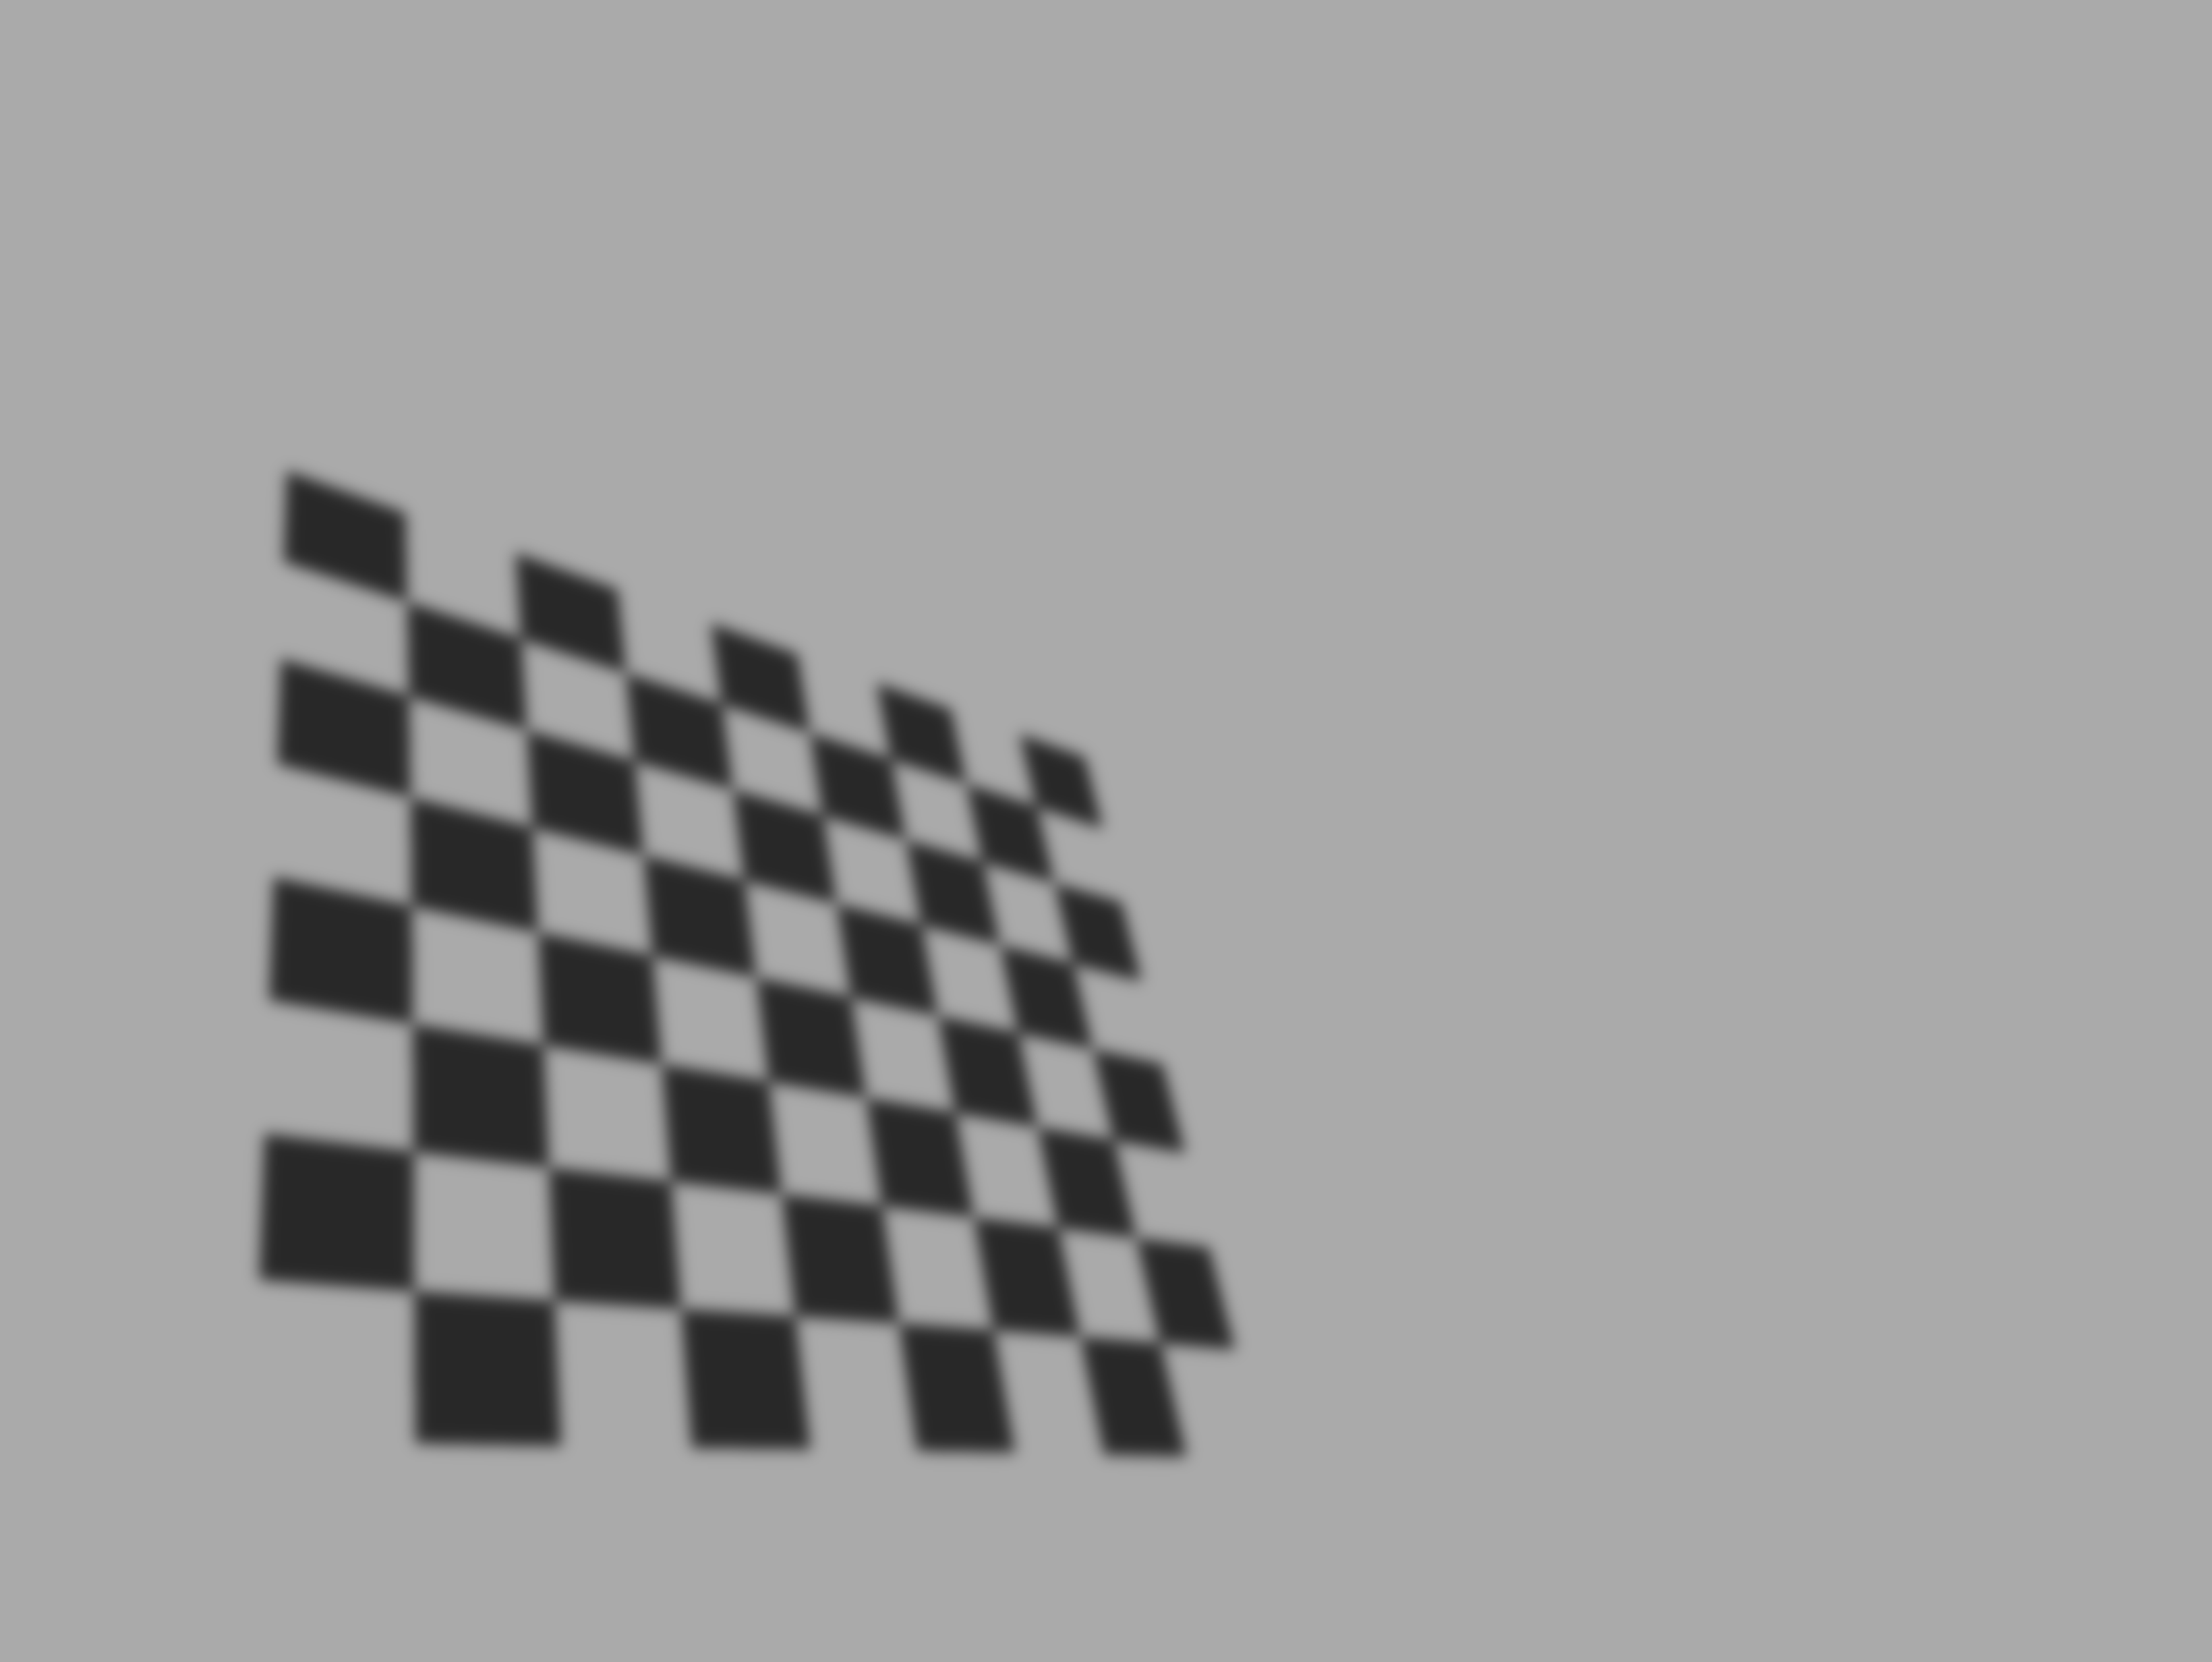
\includegraphics[width=0.9\linewidth]{3-development/calibration/images/nump1_blurred.png}
	\caption{Blurred image\label{development:nump_blurred}}
\end{figure}
With these blurred images, it is still possible to obtain a good calibration as Figure \ref{development:blurred} shows.
The blue curve is again the model, the first (orange) curve is plotted with coefficients of the calibration out of the unaltered images and the second (blue) with the blurred images.
\begin{figure}[ht]
	\centering
	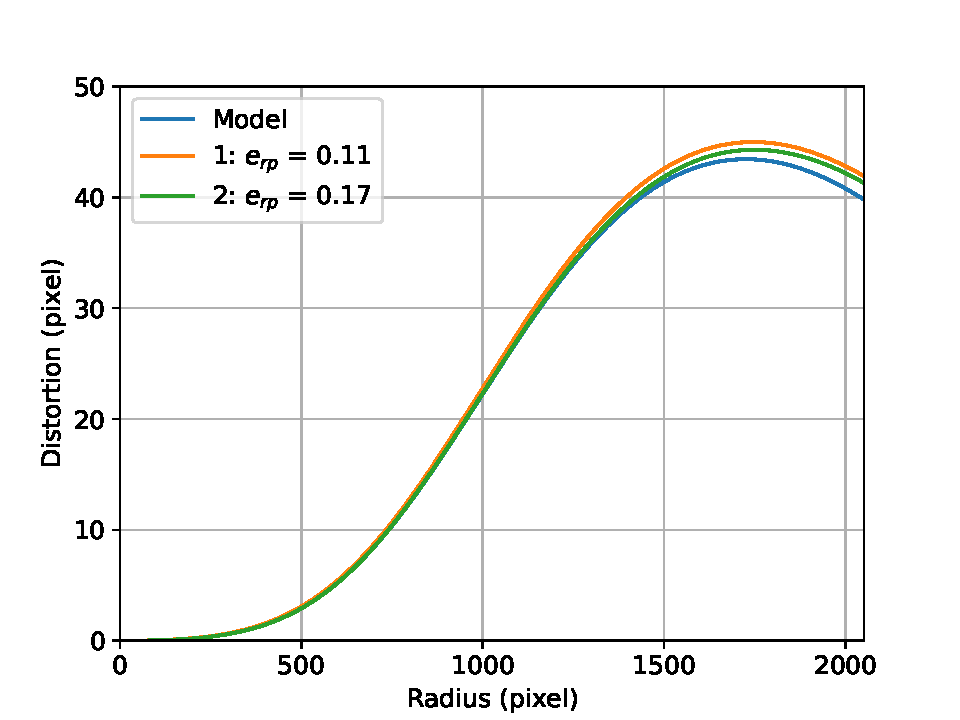
\includegraphics[width=0.9\linewidth]{3-development/calibration/images/blurred.pdf}
	\caption{Blurred calibration\label{development:blurred}}
\end{figure}
Even tough the reprojection error of the second calibration is slightly higher, it does not seem that the calibration itself is worse.
But if the images is blurred even more (with bigger size of the kernel), it is not possible to detect the checkerboard corners.
Images which are not sharp, do therefore not affect the calibration, since slightly blurred images do not make the calibration worse, and strongly blurred images are sorted out since no checkerboard corners can be detected.

\subsubsection{Summary}
Concerning the images used for the calibration, the most important insights are:
\begin{itemize}
\item Including images, with checkerboard corners close to the edges makes the calibration much more stable.
\item Noise should be kept as low as possible. To ensure this, one should try to get as much light on the sensor of the camera, so that the automatic exposure control can reduce the ISO to a minimum.
\item Blurred images do not affect the calibration. But since the blurry images are sorted out, it is necessary to have a certain amount of good images.
\end{itemize}
By taking these points into account, it should be possible to obtain the optimal calibration with the introduced methods.


\subsection{Fixed calibration}
Following table displays the best possible set of coefficients with their corresponding standard deviation obtained before taking all the learned points into account, denoted with the superscript $(1)$.
\begin{center}
	\begin{tabular}{lll}
		$k_1^{(1)}=3.0\pm 5.1$&$k_2^{(1)}=44.3\pm 7.5$&$k_3^{(1)}=-17.0\pm 77.6$\\
		$k_4^{(1)}=3.0\pm 5.2$&$k_5^{(1)}=42.5\pm 8.0$&$k_6^{(1)}=-14.2\pm 77.8$\\
		$p_1^{(1)}=0.0017\pm 0.0006$&$p_2^{(1)}=0.0037\pm 0.0006$&$s_1^{(1)}=-0.0032\pm 0.005$\\
		$s_2^{(1)}=-0.0032\pm 0.0013$&$s_2^{(1)}=-0.0022\pm 0.0005$&$s_4^{(1)}=0.0014\pm 0.0010$
	\end{tabular} 
\end{center}
The reprojection error is $e_{\text{rp}}^{(1)}=0.324$.
The problem with this calibration is visible when looking at the standard deviations, which are way to high, especially by the radial distortion coefficients.
But again these coefficients will dominate the whole calibration.

The next table then shows the best possible calibration coefficients when considering all new insights, denoted with the superscript $(2)$.
\begin{center}
	\begin{tabular}{lll}
		$k_1^{(2)}=18.2\pm1.2$&$k_2^{(2)}=15.7\pm5.2$&$k_3^{(2)}=234.7\pm0.2$\\
		$k_4^{(2)}=18.2\pm1.2$&$k_5^{(2)}=12.1\pm4.9$&$k_6^{(2)}=236.9\pm0.5$\\
		$p_1^{(2)}=-0.0031\pm0.0004$&$p_2^{(2)}=0.000013\pm0.00028$&$s_1^{(2)}=0.00064\pm0.00024$\\
		$s_2^{(2)}=-0.0018\pm0.0006$&$s_3^{(2)}=0.0047\pm0.0004$&$s_4^{(2)}=-0.0013\pm 0.0006$
	\end{tabular}		
\end{center}
With this calibration we get a reprojection error $e_{\text{rp}}^{(2)}$ of 0.287.
The standard deviations are (excluding $p_2$ and $s_1$) at least on order of magnitude smaller than the coefficient itself.
This is seems something better than before, but since this error is a training error, we can not tell if this really performs better.

We now use the method suggested in section \ref{theory:error_propagation} to combine all these standard deviations into one value in dependence of the radius.
This will give us an additional value on which base we can asses the quality of the calibration. 
With the resolution set to $3280\times 2464$\,pixels, we get at the maximum radius a standard deviation of $\Delta r^{(1)}(2051)=2464\,$pixels ind the first case, and $\Delta r^{(2)}(2051)=72\,$pixels in the fixed calibration.

If we applied this calibration, our standard deviation in the image corners would (especially in the first case) be much lower than these value.
But the propagation of error is a linearization of the non-linear calibration model in equation \ref{theory:dist} and adds up all errors.
Despite all of this, when looking at the to uncertainties ($\Delta r^{(1)}(r)$ and $\Delta r^{(2)}(r)$) that the second, fixed calibration seems to perform much better.
How much is hard to say, again because we are working with linearization.
the only thing we can safely say is, that the second calibration does a better job than the first, but we have no quantity to estimate how much better.

Nevertheless, it is reasonable to use this second calibration, since we included all our gained knowledge into it.
It may be possible to obtain a better results by detecting the checkerboard differently (without OpneCV), but this is not in the scope of this thesis. 